% Options for packages loaded elsewhere
\PassOptionsToPackage{unicode}{hyperref}
\PassOptionsToPackage{hyphens}{url}
%
\documentclass[
]{article}
\usepackage{amsmath,amssymb}
\usepackage{lmodern}
\usepackage{ifxetex,ifluatex}
\ifnum 0\ifxetex 1\fi\ifluatex 1\fi=0 % if pdftex
  \usepackage[T1]{fontenc}
  \usepackage[utf8]{inputenc}
  \usepackage{textcomp} % provide euro and other symbols
\else % if luatex or xetex
  \usepackage{unicode-math}
  \defaultfontfeatures{Scale=MatchLowercase}
  \defaultfontfeatures[\rmfamily]{Ligatures=TeX,Scale=1}
\fi
% Use upquote if available, for straight quotes in verbatim environments
\IfFileExists{upquote.sty}{\usepackage{upquote}}{}
\IfFileExists{microtype.sty}{% use microtype if available
  \usepackage[]{microtype}
  \UseMicrotypeSet[protrusion]{basicmath} % disable protrusion for tt fonts
}{}
\makeatletter
\@ifundefined{KOMAClassName}{% if non-KOMA class
  \IfFileExists{parskip.sty}{%
    \usepackage{parskip}
  }{% else
    \setlength{\parindent}{0pt}
    \setlength{\parskip}{6pt plus 2pt minus 1pt}}
}{% if KOMA class
  \KOMAoptions{parskip=half}}
\makeatother
\usepackage{xcolor}
\IfFileExists{xurl.sty}{\usepackage{xurl}}{} % add URL line breaks if available
\IfFileExists{bookmark.sty}{\usepackage{bookmark}}{\usepackage{hyperref}}
\hypersetup{
  pdftitle={621\_Final\_HomeSales},
  pdfauthor={Eric Hirsch, Cameron Smith and Carlisle Fergusen},
  hidelinks,
  pdfcreator={LaTeX via pandoc}}
\urlstyle{same} % disable monospaced font for URLs
\usepackage[margin=1in]{geometry}
\usepackage{graphicx}
\makeatletter
\def\maxwidth{\ifdim\Gin@nat@width>\linewidth\linewidth\else\Gin@nat@width\fi}
\def\maxheight{\ifdim\Gin@nat@height>\textheight\textheight\else\Gin@nat@height\fi}
\makeatother
% Scale images if necessary, so that they will not overflow the page
% margins by default, and it is still possible to overwrite the defaults
% using explicit options in \includegraphics[width, height, ...]{}
\setkeys{Gin}{width=\maxwidth,height=\maxheight,keepaspectratio}
% Set default figure placement to htbp
\makeatletter
\def\fps@figure{htbp}
\makeatother
\setlength{\emergencystretch}{3em} % prevent overfull lines
\providecommand{\tightlist}{%
  \setlength{\itemsep}{0pt}\setlength{\parskip}{0pt}}
\setcounter{secnumdepth}{-\maxdimen} % remove section numbering
\usepackage{setspace}\doublespacing
\ifluatex
  \usepackage{selnolig}  % disable illegal ligatures
\fi

\title{621\_Final\_HomeSales}
\author{Eric Hirsch, Cameron Smith and Carlisle Fergusen}
\date{4/7/2022}

\begin{document}
\maketitle

{
\setcounter{tocdepth}{4}
\tableofcontents
}
\hypertarget{abstract}{%
\subsection{\texorpdfstring{\emph{Abstract}}{Abstract}}\label{abstract}}

Being able to accurately predict housing prices is critical to many
industries. Recently, analysts have attempted to improve price
prediction with enhanced statistical techniques. In this paper, we take
a more comparative approach, examining 4 standard regression techniques
(OLS, ridge lasso, and elastic net) to assess the best performance. We
used a kaggle dataset
(\url{https://www.kaggle.com/c/house-prices-advanced-regression-techniques})
in order to test the performance of the model. We found Lasso to be the
best predictor, which we speculate is because the dataset has a high
number of predictors relative to the number of observations.

\hypertarget{introduction}{%
\subsection{\texorpdfstring{\emph{Introduction}}{Introduction}}\label{introduction}}

In this paper we analyze housing prices by comparing three prediction
methodologies: OLS, Ridge regression, and Random Forest. The purpose is
to compare the methodologies and draw conclusions about which are most
effective and why. Regression alone is not necessarily the optimal
strategy for predicting housing prices.\footnote{1 Prediction of China's
  Housing Price Based on a Novel Grey Seasonal Model, Li et
  al.~Mathematical Models in Engineering,
  \url{https://www.hindawi.com/journals/mpe/2021/5541233/}} However,
when data sets and/or analysis resources are limited, regression can
perform adequately.

\hypertarget{background-and-literature-review}{%
\subsection{\texorpdfstring{\emph{Background and Literature
Review}}{Background and Literature Review}}\label{background-and-literature-review}}

The ability to accurately predict home prices is of tremendous value to
a number of industries, including investors, real estate agents, and
municipalities who depend upon property tax revenue. ¹ Predictive models
for home prices fall roughly into two kinds. First, there are those
which predict market trends, busts, and booms. These predictions rely
mainly on timeseries data and analysis of housing prices in the
aggregate. The other type of prediction involves the capacity to predict
individual house prices from a set of factors. These usually employ some
form of regression and/or machine learning.\footnote{2}

For either sort of prediction, there is no consensus about the best
method. Many researchers have sought to enhance the traditional models
with other methodologies.\footnote{3} For example, Guan et. al.~propose
a ``data stream'' approach in which past sale records are treated as an
evolving datastream.\footnote{4} Li et. al.~introduce a ``grey seasonal
model'' in which seasonal fluctuations are modeled using grey systems
theory, which incorporates uncertainty.\footnote{5} Alfiyatin, et. el.
use particle swarm optimization (PSO) to select independent
variables.\footnote{6} (PSO is an optimization system in which
population is initialized with random solutions and searches for optima
by updating generations.) Finally, Liu et.al incorporate both spatial
and temporal autocorrelation in their models by analyzing
experience-based submarkets by real estate professionals.\footnote{7}

All of these researchers report that their innovations improve their
regression models. Indeed, any real estate agent can tell you that a
predictive model can be improved simply by knowing what other houses in
the neighborhood sold for. The problem is, the data at the center of
these enhancements is not always available. The researcher may have home
sales from only a short time span, and neighborhoods that are not
defined by real estate experts but by traditional boundary lines which
may contain a mix of house types. Even when data is available, the
complex models proposed may be computationally expensive and/or require
data analysis expertise that is not generally available.

In this project we approach the question comparatively. Restricting
ourselves to regression models, we compare three types of regression:
OLS, Ridge, and Random Forest. At the data is drawn from the Advanced
Regression Techniques housing data set for Ames, Iowa. We test the
accuracy of our models by submitting each to the Kaggle competition to
see how they perform. We then discussed the merits of the different
sorts of approaches.

\hypertarget{modeling}{%
\subsection{\texorpdfstring{\emph{Modeling}}{Modeling}}\label{modeling}}

We are modeling a data set containing 1460 records of houses sold in the
Ames, Iowa area between 2006 and 2010. The variables are mostly related
to house features, such as square footage, the presense of a pool, etc.
The response variable, ``SalePrice'', is a continuous variable
representing the sale price of the house in dollars.

We examine the data:

\hypertarget{dataset-description}{%
\subsubsection{1. Dataset Description}\label{dataset-description}}

\hypertarget{a.-summary-statistics}{%
\paragraph{A. Summary Statistics}\label{a.-summary-statistics}}

\begin{verbatim}
##        Id           MSSubClass       MSZoning     LotFrontage    
##  Min.   :   1.0   Min.   : 20.0   C (all):  10   Min.   : 21.00  
##  1st Qu.: 365.8   1st Qu.: 20.0   FV     :  65   1st Qu.: 59.00  
##  Median : 730.5   Median : 50.0   RH     :  16   Median : 69.00  
##  Mean   : 730.5   Mean   : 56.9   RL     :1151   Mean   : 70.05  
##  3rd Qu.:1095.2   3rd Qu.: 70.0   RM     : 218   3rd Qu.: 80.00  
##  Max.   :1460.0   Max.   :190.0                  Max.   :313.00  
##                                                  NA's   :259     
##     LotArea        Street      Alley      LotShape  LandContour  Utilities   
##  Min.   :  1300   Grvl:   6   Grvl:  50   IR1:484   Bnk:  63    AllPub:1459  
##  1st Qu.:  7554   Pave:1454   Pave:  41   IR2: 41   HLS:  50    NoSeWa:   1  
##  Median :  9478               NA's:1369   IR3: 10   Low:  36                 
##  Mean   : 10517                           Reg:925   Lvl:1311                 
##  3rd Qu.: 11602                                                              
##  Max.   :215245                                                              
##                                                                              
##    LotConfig    LandSlope   Neighborhood   Condition1     Condition2  
##  Corner : 263   Gtl:1382   NAmes  :225   Norm   :1260   Norm   :1445  
##  CulDSac:  94   Mod:  65   CollgCr:150   Feedr  :  81   Feedr  :   6  
##  FR2    :  47   Sev:  13   OldTown:113   Artery :  48   Artery :   2  
##  FR3    :   4              Edwards:100   RRAn   :  26   PosN   :   2  
##  Inside :1052              Somerst: 86   PosN   :  19   RRNn   :   2  
##                            Gilbert: 79   RRAe   :  11   PosA   :   1  
##                            (Other):707   (Other):  15   (Other):   2  
##    BldgType      HouseStyle   OverallQual      OverallCond      YearBuilt   
##  1Fam  :1220   1Story :726   Min.   : 1.000   Min.   :1.000   Min.   :1872  
##  2fmCon:  31   2Story :445   1st Qu.: 5.000   1st Qu.:5.000   1st Qu.:1954  
##  Duplex:  52   1.5Fin :154   Median : 6.000   Median :5.000   Median :1973  
##  Twnhs :  43   SLvl   : 65   Mean   : 6.099   Mean   :5.575   Mean   :1971  
##  TwnhsE: 114   SFoyer : 37   3rd Qu.: 7.000   3rd Qu.:6.000   3rd Qu.:2000  
##                1.5Unf : 14   Max.   :10.000   Max.   :9.000   Max.   :2010  
##                (Other): 19                                                  
##   YearRemodAdd    RoofStyle       RoofMatl     Exterior1st   Exterior2nd 
##  Min.   :1950   Flat   :  13   CompShg:1434   VinylSd:515   VinylSd:504  
##  1st Qu.:1967   Gable  :1141   Tar&Grv:  11   HdBoard:222   MetalSd:214  
##  Median :1994   Gambrel:  11   WdShngl:   6   MetalSd:220   HdBoard:207  
##  Mean   :1985   Hip    : 286   WdShake:   5   Wd Sdng:206   Wd Sdng:197  
##  3rd Qu.:2004   Mansard:   7   ClyTile:   1   Plywood:108   Plywood:142  
##  Max.   :2010   Shed   :   2   Membran:   1   CemntBd: 61   CmentBd: 60  
##                                (Other):   2   (Other):128   (Other):136  
##    MasVnrType    MasVnrArea     ExterQual ExterCond  Foundation  BsmtQual  
##  BrkCmn : 15   Min.   :   0.0   Ex: 52    Ex:   3   BrkTil:146   Ex  :121  
##  BrkFace:445   1st Qu.:   0.0   Fa: 14    Fa:  28   CBlock:634   Fa  : 35  
##  None   :864   Median :   0.0   Gd:488    Gd: 146   PConc :647   Gd  :618  
##  Stone  :128   Mean   : 103.7   TA:906    Po:   1   Slab  : 24   TA  :649  
##  NA's   :  8   3rd Qu.: 166.0             TA:1282   Stone :  6   NA's: 37  
##                Max.   :1600.0                       Wood  :  3             
##                NA's   :8                                                   
##  BsmtCond    BsmtExposure BsmtFinType1   BsmtFinSF1     BsmtFinType2
##  Fa  :  45   Av  :221     ALQ :220     Min.   :   0.0   ALQ :  19   
##  Gd  :  65   Gd  :134     BLQ :148     1st Qu.:   0.0   BLQ :  33   
##  Po  :   2   Mn  :114     GLQ :418     Median : 383.5   GLQ :  14   
##  TA  :1311   No  :953     LwQ : 74     Mean   : 443.6   LwQ :  46   
##  NA's:  37   NA's: 38     Rec :133     3rd Qu.: 712.2   Rec :  54   
##                           Unf :430     Max.   :5644.0   Unf :1256   
##                           NA's: 37                      NA's:  38   
##    BsmtFinSF2        BsmtUnfSF       TotalBsmtSF      Heating     HeatingQC
##  Min.   :   0.00   Min.   :   0.0   Min.   :   0.0   Floor:   1   Ex:741   
##  1st Qu.:   0.00   1st Qu.: 223.0   1st Qu.: 795.8   GasA :1428   Fa: 49   
##  Median :   0.00   Median : 477.5   Median : 991.5   GasW :  18   Gd:241   
##  Mean   :  46.55   Mean   : 567.2   Mean   :1057.4   Grav :   7   Po:  1   
##  3rd Qu.:   0.00   3rd Qu.: 808.0   3rd Qu.:1298.2   OthW :   2   TA:428   
##  Max.   :1474.00   Max.   :2336.0   Max.   :6110.0   Wall :   4            
##                                                                            
##  CentralAir Electrical     X1stFlrSF      X2ndFlrSF     LowQualFinSF    
##  N:  95     FuseA:  94   Min.   : 334   Min.   :   0   Min.   :  0.000  
##  Y:1365     FuseF:  27   1st Qu.: 882   1st Qu.:   0   1st Qu.:  0.000  
##             FuseP:   3   Median :1087   Median :   0   Median :  0.000  
##             Mix  :   1   Mean   :1163   Mean   : 347   Mean   :  5.845  
##             SBrkr:1334   3rd Qu.:1391   3rd Qu.: 728   3rd Qu.:  0.000  
##             NA's :   1   Max.   :4692   Max.   :2065   Max.   :572.000  
##                                                                         
##    GrLivArea     BsmtFullBath     BsmtHalfBath        FullBath    
##  Min.   : 334   Min.   :0.0000   Min.   :0.00000   Min.   :0.000  
##  1st Qu.:1130   1st Qu.:0.0000   1st Qu.:0.00000   1st Qu.:1.000  
##  Median :1464   Median :0.0000   Median :0.00000   Median :2.000  
##  Mean   :1515   Mean   :0.4253   Mean   :0.05753   Mean   :1.565  
##  3rd Qu.:1777   3rd Qu.:1.0000   3rd Qu.:0.00000   3rd Qu.:2.000  
##  Max.   :5642   Max.   :3.0000   Max.   :2.00000   Max.   :3.000  
##                                                                   
##     HalfBath       BedroomAbvGr    KitchenAbvGr   KitchenQual  TotRmsAbvGrd   
##  Min.   :0.0000   Min.   :0.000   Min.   :0.000   Ex:100      Min.   : 2.000  
##  1st Qu.:0.0000   1st Qu.:2.000   1st Qu.:1.000   Fa: 39      1st Qu.: 5.000  
##  Median :0.0000   Median :3.000   Median :1.000   Gd:586      Median : 6.000  
##  Mean   :0.3829   Mean   :2.866   Mean   :1.047   TA:735      Mean   : 6.518  
##  3rd Qu.:1.0000   3rd Qu.:3.000   3rd Qu.:1.000               3rd Qu.: 7.000  
##  Max.   :2.0000   Max.   :8.000   Max.   :3.000               Max.   :14.000  
##                                                                               
##  Functional    Fireplaces    FireplaceQu   GarageType   GarageYrBlt  
##  Maj1:  14   Min.   :0.000   Ex  : 24    2Types :  6   Min.   :1900  
##  Maj2:   5   1st Qu.:0.000   Fa  : 33    Attchd :870   1st Qu.:1961  
##  Min1:  31   Median :1.000   Gd  :380    Basment: 19   Median :1980  
##  Min2:  34   Mean   :0.613   Po  : 20    BuiltIn: 88   Mean   :1979  
##  Mod :  15   3rd Qu.:1.000   TA  :313    CarPort:  9   3rd Qu.:2002  
##  Sev :   1   Max.   :3.000   NA's:690    Detchd :387   Max.   :2010  
##  Typ :1360                               NA's   : 81   NA's   :81    
##  GarageFinish   GarageCars      GarageArea     GarageQual  GarageCond 
##  Fin :352     Min.   :0.000   Min.   :   0.0   Ex  :   3   Ex  :   2  
##  RFn :422     1st Qu.:1.000   1st Qu.: 334.5   Fa  :  48   Fa  :  35  
##  Unf :605     Median :2.000   Median : 480.0   Gd  :  14   Gd  :   9  
##  NA's: 81     Mean   :1.767   Mean   : 473.0   Po  :   3   Po  :   7  
##               3rd Qu.:2.000   3rd Qu.: 576.0   TA  :1311   TA  :1326  
##               Max.   :4.000   Max.   :1418.0   NA's:  81   NA's:  81  
##                                                                       
##  PavedDrive   WoodDeckSF      OpenPorchSF     EnclosedPorch      X3SsnPorch    
##  N:  90     Min.   :  0.00   Min.   :  0.00   Min.   :  0.00   Min.   :  0.00  
##  P:  30     1st Qu.:  0.00   1st Qu.:  0.00   1st Qu.:  0.00   1st Qu.:  0.00  
##  Y:1340     Median :  0.00   Median : 25.00   Median :  0.00   Median :  0.00  
##             Mean   : 94.24   Mean   : 46.66   Mean   : 21.95   Mean   :  3.41  
##             3rd Qu.:168.00   3rd Qu.: 68.00   3rd Qu.:  0.00   3rd Qu.:  0.00  
##             Max.   :857.00   Max.   :547.00   Max.   :552.00   Max.   :508.00  
##                                                                                
##   ScreenPorch        PoolArea        PoolQC       Fence      MiscFeature
##  Min.   :  0.00   Min.   :  0.000   Ex  :   2   GdPrv:  59   Gar2:   2  
##  1st Qu.:  0.00   1st Qu.:  0.000   Fa  :   2   GdWo :  54   Othr:   2  
##  Median :  0.00   Median :  0.000   Gd  :   3   MnPrv: 157   Shed:  49  
##  Mean   : 15.06   Mean   :  2.759   NA's:1453   MnWw :  11   TenC:   1  
##  3rd Qu.:  0.00   3rd Qu.:  0.000               NA's :1179   NA's:1406  
##  Max.   :480.00   Max.   :738.000                                       
##                                                                         
##     MiscVal             MoSold           YrSold        SaleType   
##  Min.   :    0.00   Min.   : 1.000   Min.   :2006   WD     :1267  
##  1st Qu.:    0.00   1st Qu.: 5.000   1st Qu.:2007   New    : 122  
##  Median :    0.00   Median : 6.000   Median :2008   COD    :  43  
##  Mean   :   43.49   Mean   : 6.322   Mean   :2008   ConLD  :   9  
##  3rd Qu.:    0.00   3rd Qu.: 8.000   3rd Qu.:2009   ConLI  :   5  
##  Max.   :15500.00   Max.   :12.000   Max.   :2010   ConLw  :   5  
##                                                     (Other):   9  
##  SaleCondition    SalePrice     
##  Abnorml: 101   Min.   : 34900  
##  AdjLand:   4   1st Qu.:129975  
##  Alloca :  12   Median :163000  
##  Family :  20   Mean   :180921  
##  Normal :1198   3rd Qu.:214000  
##  Partial: 125   Max.   :755000  
## 
\end{verbatim}

\begin{verbatim}
## 'data.frame':    1460 obs. of  81 variables:
##  $ Id           : int  1 2 3 4 5 6 7 8 9 10 ...
##  $ MSSubClass   : int  60 20 60 70 60 50 20 60 50 190 ...
##  $ MSZoning     : Factor w/ 5 levels "C (all)","FV",..: 4 4 4 4 4 4 4 4 5 4 ...
##  $ LotFrontage  : int  65 80 68 60 84 85 75 NA 51 50 ...
##  $ LotArea      : int  8450 9600 11250 9550 14260 14115 10084 10382 6120 7420 ...
##  $ Street       : Factor w/ 2 levels "Grvl","Pave": 2 2 2 2 2 2 2 2 2 2 ...
##  $ Alley        : Factor w/ 2 levels "Grvl","Pave": NA NA NA NA NA NA NA NA NA NA ...
##  $ LotShape     : Factor w/ 4 levels "IR1","IR2","IR3",..: 4 4 1 1 1 1 4 1 4 4 ...
##  $ LandContour  : Factor w/ 4 levels "Bnk","HLS","Low",..: 4 4 4 4 4 4 4 4 4 4 ...
##  $ Utilities    : Factor w/ 2 levels "AllPub","NoSeWa": 1 1 1 1 1 1 1 1 1 1 ...
##  $ LotConfig    : Factor w/ 5 levels "Corner","CulDSac",..: 5 3 5 1 3 5 5 1 5 1 ...
##  $ LandSlope    : Factor w/ 3 levels "Gtl","Mod","Sev": 1 1 1 1 1 1 1 1 1 1 ...
##  $ Neighborhood : Factor w/ 25 levels "Blmngtn","Blueste",..: 6 25 6 7 14 12 21 17 18 4 ...
##  $ Condition1   : Factor w/ 9 levels "Artery","Feedr",..: 3 2 3 3 3 3 3 5 1 1 ...
##  $ Condition2   : Factor w/ 8 levels "Artery","Feedr",..: 3 3 3 3 3 3 3 3 3 1 ...
##  $ BldgType     : Factor w/ 5 levels "1Fam","2fmCon",..: 1 1 1 1 1 1 1 1 1 2 ...
##  $ HouseStyle   : Factor w/ 8 levels "1.5Fin","1.5Unf",..: 6 3 6 6 6 1 3 6 1 2 ...
##  $ OverallQual  : int  7 6 7 7 8 5 8 7 7 5 ...
##  $ OverallCond  : int  5 8 5 5 5 5 5 6 5 6 ...
##  $ YearBuilt    : int  2003 1976 2001 1915 2000 1993 2004 1973 1931 1939 ...
##  $ YearRemodAdd : int  2003 1976 2002 1970 2000 1995 2005 1973 1950 1950 ...
##  $ RoofStyle    : Factor w/ 6 levels "Flat","Gable",..: 2 2 2 2 2 2 2 2 2 2 ...
##  $ RoofMatl     : Factor w/ 8 levels "ClyTile","CompShg",..: 2 2 2 2 2 2 2 2 2 2 ...
##  $ Exterior1st  : Factor w/ 15 levels "AsbShng","AsphShn",..: 13 9 13 14 13 13 13 7 4 9 ...
##  $ Exterior2nd  : Factor w/ 16 levels "AsbShng","AsphShn",..: 14 9 14 16 14 14 14 7 16 9 ...
##  $ MasVnrType   : Factor w/ 4 levels "BrkCmn","BrkFace",..: 2 3 2 3 2 3 4 4 3 3 ...
##  $ MasVnrArea   : int  196 0 162 0 350 0 186 240 0 0 ...
##  $ ExterQual    : Factor w/ 4 levels "Ex","Fa","Gd",..: 3 4 3 4 3 4 3 4 4 4 ...
##  $ ExterCond    : Factor w/ 5 levels "Ex","Fa","Gd",..: 5 5 5 5 5 5 5 5 5 5 ...
##  $ Foundation   : Factor w/ 6 levels "BrkTil","CBlock",..: 3 2 3 1 3 6 3 2 1 1 ...
##  $ BsmtQual     : Factor w/ 4 levels "Ex","Fa","Gd",..: 3 3 3 4 3 3 1 3 4 4 ...
##  $ BsmtCond     : Factor w/ 4 levels "Fa","Gd","Po",..: 4 4 4 2 4 4 4 4 4 4 ...
##  $ BsmtExposure : Factor w/ 4 levels "Av","Gd","Mn",..: 4 2 3 4 1 4 1 3 4 4 ...
##  $ BsmtFinType1 : Factor w/ 6 levels "ALQ","BLQ","GLQ",..: 3 1 3 1 3 3 3 1 6 3 ...
##  $ BsmtFinSF1   : int  706 978 486 216 655 732 1369 859 0 851 ...
##  $ BsmtFinType2 : Factor w/ 6 levels "ALQ","BLQ","GLQ",..: 6 6 6 6 6 6 6 2 6 6 ...
##  $ BsmtFinSF2   : int  0 0 0 0 0 0 0 32 0 0 ...
##  $ BsmtUnfSF    : int  150 284 434 540 490 64 317 216 952 140 ...
##  $ TotalBsmtSF  : int  856 1262 920 756 1145 796 1686 1107 952 991 ...
##  $ Heating      : Factor w/ 6 levels "Floor","GasA",..: 2 2 2 2 2 2 2 2 2 2 ...
##  $ HeatingQC    : Factor w/ 5 levels "Ex","Fa","Gd",..: 1 1 1 3 1 1 1 1 3 1 ...
##  $ CentralAir   : Factor w/ 2 levels "N","Y": 2 2 2 2 2 2 2 2 2 2 ...
##  $ Electrical   : Factor w/ 5 levels "FuseA","FuseF",..: 5 5 5 5 5 5 5 5 2 5 ...
##  $ X1stFlrSF    : int  856 1262 920 961 1145 796 1694 1107 1022 1077 ...
##  $ X2ndFlrSF    : int  854 0 866 756 1053 566 0 983 752 0 ...
##  $ LowQualFinSF : int  0 0 0 0 0 0 0 0 0 0 ...
##  $ GrLivArea    : int  1710 1262 1786 1717 2198 1362 1694 2090 1774 1077 ...
##  $ BsmtFullBath : int  1 0 1 1 1 1 1 1 0 1 ...
##  $ BsmtHalfBath : int  0 1 0 0 0 0 0 0 0 0 ...
##  $ FullBath     : int  2 2 2 1 2 1 2 2 2 1 ...
##  $ HalfBath     : int  1 0 1 0 1 1 0 1 0 0 ...
##  $ BedroomAbvGr : int  3 3 3 3 4 1 3 3 2 2 ...
##  $ KitchenAbvGr : int  1 1 1 1 1 1 1 1 2 2 ...
##  $ KitchenQual  : Factor w/ 4 levels "Ex","Fa","Gd",..: 3 4 3 3 3 4 3 4 4 4 ...
##  $ TotRmsAbvGrd : int  8 6 6 7 9 5 7 7 8 5 ...
##  $ Functional   : Factor w/ 7 levels "Maj1","Maj2",..: 7 7 7 7 7 7 7 7 3 7 ...
##  $ Fireplaces   : int  0 1 1 1 1 0 1 2 2 2 ...
##  $ FireplaceQu  : Factor w/ 5 levels "Ex","Fa","Gd",..: NA 5 5 3 5 NA 3 5 5 5 ...
##  $ GarageType   : Factor w/ 6 levels "2Types","Attchd",..: 2 2 2 6 2 2 2 2 6 2 ...
##  $ GarageYrBlt  : int  2003 1976 2001 1998 2000 1993 2004 1973 1931 1939 ...
##  $ GarageFinish : Factor w/ 3 levels "Fin","RFn","Unf": 2 2 2 3 2 3 2 2 3 2 ...
##  $ GarageCars   : int  2 2 2 3 3 2 2 2 2 1 ...
##  $ GarageArea   : int  548 460 608 642 836 480 636 484 468 205 ...
##  $ GarageQual   : Factor w/ 5 levels "Ex","Fa","Gd",..: 5 5 5 5 5 5 5 5 2 3 ...
##  $ GarageCond   : Factor w/ 5 levels "Ex","Fa","Gd",..: 5 5 5 5 5 5 5 5 5 5 ...
##  $ PavedDrive   : Factor w/ 3 levels "N","P","Y": 3 3 3 3 3 3 3 3 3 3 ...
##  $ WoodDeckSF   : int  0 298 0 0 192 40 255 235 90 0 ...
##  $ OpenPorchSF  : int  61 0 42 35 84 30 57 204 0 4 ...
##  $ EnclosedPorch: int  0 0 0 272 0 0 0 228 205 0 ...
##  $ X3SsnPorch   : int  0 0 0 0 0 320 0 0 0 0 ...
##  $ ScreenPorch  : int  0 0 0 0 0 0 0 0 0 0 ...
##  $ PoolArea     : int  0 0 0 0 0 0 0 0 0 0 ...
##  $ PoolQC       : Factor w/ 3 levels "Ex","Fa","Gd": NA NA NA NA NA NA NA NA NA NA ...
##  $ Fence        : Factor w/ 4 levels "GdPrv","GdWo",..: NA NA NA NA NA 3 NA NA NA NA ...
##  $ MiscFeature  : Factor w/ 4 levels "Gar2","Othr",..: NA NA NA NA NA 3 NA 3 NA NA ...
##  $ MiscVal      : int  0 0 0 0 0 700 0 350 0 0 ...
##  $ MoSold       : int  2 5 9 2 12 10 8 11 4 1 ...
##  $ YrSold       : int  2008 2007 2008 2006 2008 2009 2007 2009 2008 2008 ...
##  $ SaleType     : Factor w/ 9 levels "COD","Con","ConLD",..: 9 9 9 9 9 9 9 9 9 9 ...
##  $ SaleCondition: Factor w/ 6 levels "Abnorml","AdjLand",..: 5 5 5 1 5 5 5 5 1 5 ...
##  $ SalePrice    : int  208500 181500 223500 140000 250000 143000 307000 200000 129900 118000 ...
\end{verbatim}

The dataset consists of 1460 observations and 81 variables, some numeric
and some categorical. The target variable has a minimum of 34,950 and a
maximum of 7,550,000. The low median compared to the mean suggests some
skew.

\hypertarget{b.-missing-values}{%
\paragraph{B. Missing values}\label{b.-missing-values}}

There are missing values scattered throughout the dataset. We analyse
them:

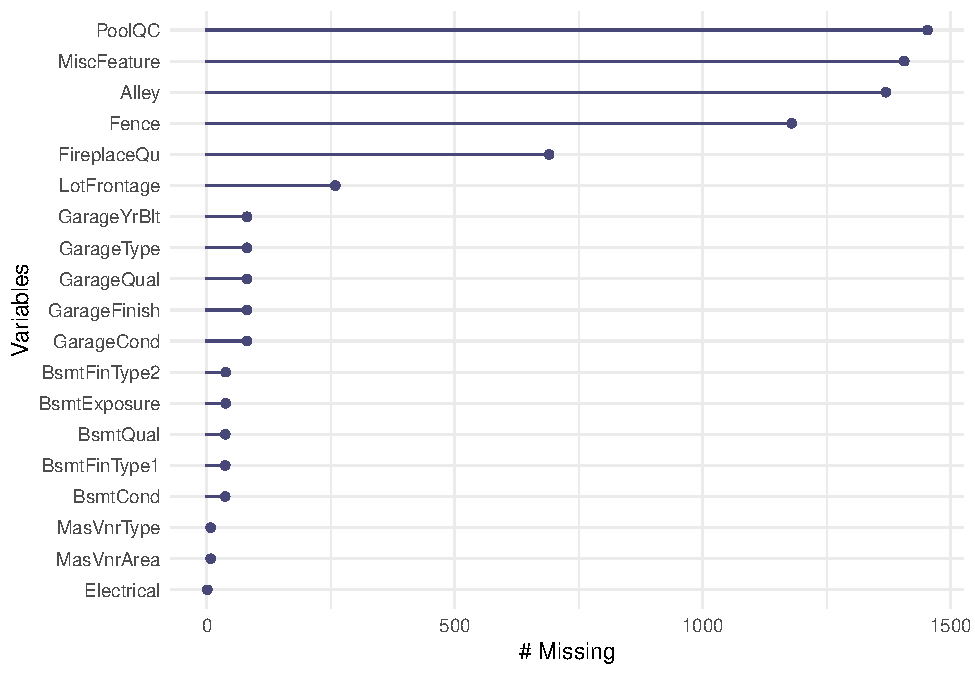
\includegraphics{Eric_Hirsch_621_Final_HomePrices_files/figure-latex/unnamed-chunk-4-1.pdf}
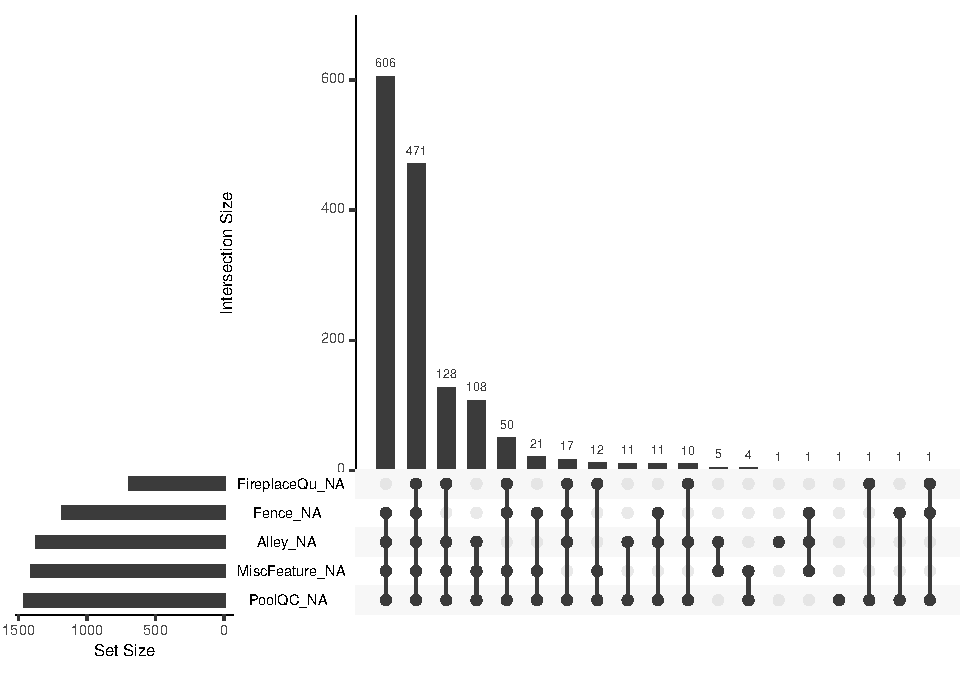
\includegraphics{Eric_Hirsch_621_Final_HomePrices_files/figure-latex/unnamed-chunk-4-2.pdf}

A few categorical features like fireplace, fence, etc. take up the bulk
of missings. They do not appear to be important enough to retain so we
delete them (FireplaceQu, Fence, Alley, MiscFeature, PoolQC, and
LotFrontage). We impute the mean for the rest.

\hypertarget{c.-create-dummy-variables}{%
\paragraph{C. Create dummy variables}\label{c.-create-dummy-variables}}

Now we create dummy variables for all of the character variables.
Categorical NA's will be handled by adding a dummy variable for NA.

\hypertarget{d.-reconcile-training-and-test-sets}{%
\paragraph{D. Reconcile training and test
sets}\label{d.-reconcile-training-and-test-sets}}

We check if the dataset is missing columns from the test dataset and if
so, drop them from the training set. This way we don't risk making
predictions on training set variables not found in the test set.

\hypertarget{e.-multicollinearity}{%
\paragraph{E. Multicollinearity}\label{e.-multicollinearity}}

We examine multicollinearity in the dataset. We look at all of the pairs
of correlations over .8 There are 24 pairs.

\begin{verbatim}
##                   col1                  col2 correlation
## 1          TotalBsmtSF             X1stFlrSF   0.8195300
## 3            GrLivArea          TotRmsAbvGrd   0.8254894
## 5           GarageCars            GarageArea   0.8824754
## 7          MSZoning_FV  Neighborhood_Somerst   0.8628071
## 9       RoofStyle_Flat      RoofMatl_Tar.Grv   0.8349139
## 11 Exterior1st_AsbShng   Exterior2nd_AsbShng   0.8479167
## 12 Exterior1st_CemntBd   Exterior2nd_CmentBd   0.9741711
## 13 Exterior1st_HdBoard   Exterior2nd_HdBoard   0.8832714
## 14 Exterior1st_MetalSd   Exterior2nd_MetalSd   0.9730652
## 15 Exterior1st_Wd.Sdng   Exterior2nd_Wd.Sdng   0.8592439
## 21     Foundation_Slab           BsmtQual_NA   0.8017334
## 22     Foundation_Slab           BsmtCond_NA   0.8017334
## 23     Foundation_Slab       BsmtFinType1_NA   0.8017334
## 25         BsmtQual_NA           BsmtCond_NA   1.0000000
## 26         BsmtQual_NA       BsmtExposure_NA   0.9864076
## 27         BsmtQual_NA       BsmtFinType1_NA   1.0000000
## 28         BsmtQual_NA       BsmtFinType2_NA   0.9864076
## 31         BsmtCond_NA       BsmtExposure_NA   0.9864076
## 32         BsmtCond_NA       BsmtFinType1_NA   1.0000000
## 33         BsmtCond_NA       BsmtFinType2_NA   0.9864076
## 36     BsmtExposure_NA       BsmtFinType1_NA   0.9864076
## 37     BsmtExposure_NA       BsmtFinType2_NA   0.9729810
## 42     BsmtFinType1_NA       BsmtFinType2_NA   0.9864076
## 47        SaleType_New SaleCondition_Partial   0.9868190
\end{verbatim}

Most of the pairs make sense - siding on the first floor will match
siding on the sencond floor, the number of cars a garage can hold will
be related to its area. We will address the multicollinearity more
closely when we run the analysis.

\hypertarget{transformations}{%
\subsubsection{2. Transformations}\label{transformations}}

\hypertarget{a.-log-of-saleprice}{%
\paragraph{A. Log of SalePrice}\label{a.-log-of-saleprice}}

The skew in the dependent variable suggests a log transformation.

\hypertarget{b.-other-transformations}{%
\paragraph{B. Other transformations}\label{b.-other-transformations}}

A number of histograms suggest issues with some of the independent
variables.

\begin{verbatim}
## [[1]]
\end{verbatim}

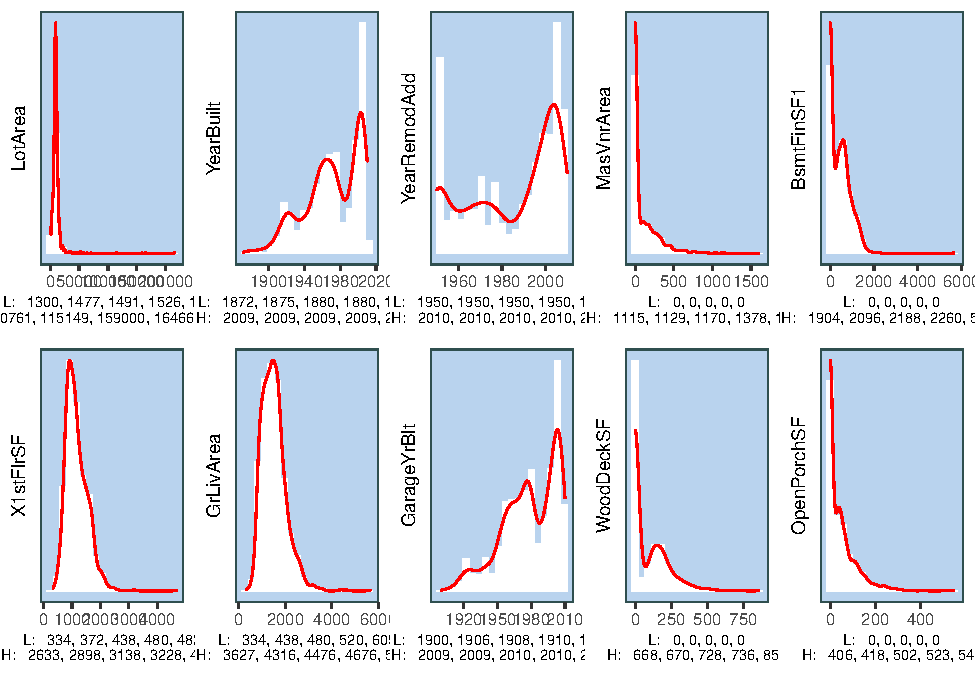
\includegraphics{Eric_Hirsch_621_Final_HomePrices_files/figure-latex/unnamed-chunk-11-1.pdf}

\begin{verbatim}
## 
## [[2]]
\end{verbatim}

\includegraphics{Eric_Hirsch_621_Final_HomePrices_files/figure-latex/unnamed-chunk-11-2.pdf}

\begin{verbatim}
## 
## [[3]]
\end{verbatim}

\includegraphics{Eric_Hirsch_621_Final_HomePrices_files/figure-latex/unnamed-chunk-11-3.pdf}

\begin{verbatim}
## 
## [[4]]
\end{verbatim}

\includegraphics{Eric_Hirsch_621_Final_HomePrices_files/figure-latex/unnamed-chunk-11-4.pdf}

\begin{verbatim}
## 
## [[5]]
\end{verbatim}

\includegraphics{Eric_Hirsch_621_Final_HomePrices_files/figure-latex/unnamed-chunk-11-5.pdf}

\begin{verbatim}
## 
## [[6]]
\end{verbatim}

\includegraphics{Eric_Hirsch_621_Final_HomePrices_files/figure-latex/unnamed-chunk-11-6.pdf}

\begin{verbatim}
## 
## [[7]]
\end{verbatim}

\includegraphics{Eric_Hirsch_621_Final_HomePrices_files/figure-latex/unnamed-chunk-11-7.pdf}

\begin{verbatim}
## 
## [[8]]
\end{verbatim}

\includegraphics{Eric_Hirsch_621_Final_HomePrices_files/figure-latex/unnamed-chunk-11-8.pdf}

\begin{verbatim}
## 
## [[9]]
\end{verbatim}

\includegraphics{Eric_Hirsch_621_Final_HomePrices_files/figure-latex/unnamed-chunk-11-9.pdf}

\begin{verbatim}
## 
## [[10]]
\end{verbatim}

\includegraphics{Eric_Hirsch_621_Final_HomePrices_files/figure-latex/unnamed-chunk-11-10.pdf}

We can see some transformations might be useful. We: 1. Add a dummy
variable to mark YearBuilt before and after 1920 2. We set YearRemodAdd
= 1950 to 0, and create a dummy variable YearRemodUnknown to track it 3.
We add dummies for NoFinBsmt, HasDeck, and HasPorch 4. We eliminate
outliers by setting LotArea\textless35000, GrLivArea3500 and
BsmtFinSF1\textless4000

\hypertarget{model-and-predict}{%
\subsubsection{3. Model and Predict:}\label{model-and-predict}}

\hypertarget{a.-base-model}{%
\paragraph{A. Base Model}\label{a.-base-model}}

We run a regression using the stepAIC algorithm to minimize AIC.

Now we make predictions

We achieve a score of .14586 on kaggle.

\hypertarget{b.-now-we-try-ridge-regression}{%
\paragraph{B. Now we try Ridge
regression:}\label{b.-now-we-try-ridge-regression}}

R makes it easy to find the best lambda by using kfold validation:

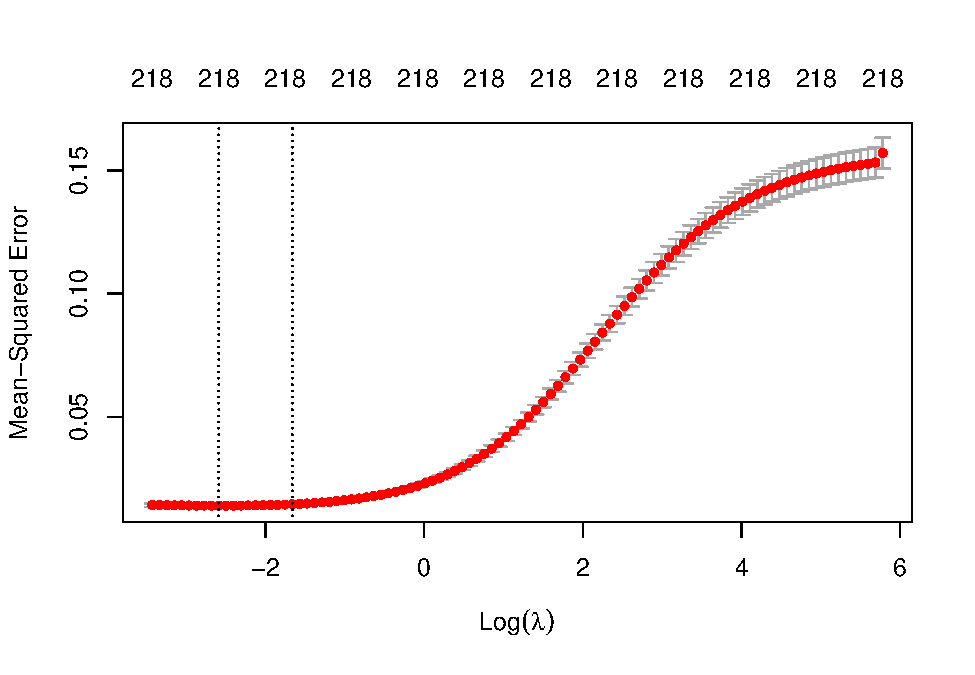
\includegraphics{Eric_Hirsch_621_Final_HomePrices_files/figure-latex/unnamed-chunk-16-1.pdf}
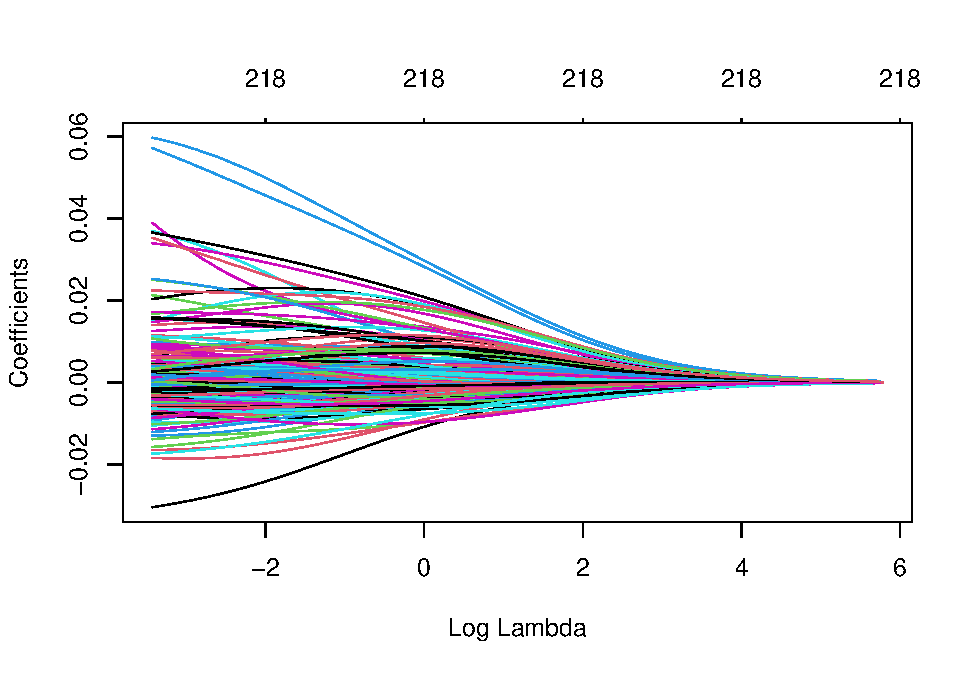
\includegraphics{Eric_Hirsch_621_Final_HomePrices_files/figure-latex/unnamed-chunk-16-2.pdf}

\begin{verbatim}
## 219 x 1 sparse Matrix of class "dgCMatrix"
##                                  s0
## (Intercept)            1.201515e+01
## Id                    -3.095103e-03
## MSSubClass             1.674301e-04
## LotArea                1.743507e-02
## OverallQual            5.270187e-02
## OverallCond            3.008382e-02
## YearBuilt              2.726814e-02
## YearRemodAdd           8.461117e-03
## MasVnrArea             4.877090e-03
## BsmtFinSF1             2.253860e-02
## BsmtFinSF2             2.488820e-03
## BsmtUnfSF              6.351351e-03
## TotalBsmtSF            3.110349e-02
## X1stFlrSF              3.116079e-02
## X2ndFlrSF              2.789420e-02
## LowQualFinSF          -5.438415e-04
## GrLivArea              4.773101e-02
## BsmtFullBath           1.472426e-02
## BsmtHalfBath           8.614658e-04
## FullBath               2.287014e-02
## HalfBath               1.522992e-02
## BedroomAbvGr           2.581921e-03
## KitchenAbvGr          -1.182839e-02
## TotRmsAbvGrd           1.933379e-02
## Fireplaces             1.600322e-02
## GarageYrBlt            1.046666e-02
## GarageCars             2.071172e-02
## GarageArea             1.759566e-02
## WoodDeckSF             9.044396e-03
## OpenPorchSF            5.548067e-03
## EnclosedPorch          4.995302e-03
## X3SsnPorch             5.610108e-03
## ScreenPorch            9.997393e-03
## PoolArea               5.208015e-03
## MiscVal               -1.583353e-03
## MoSold                 8.153092e-05
## YrSold                -1.335824e-03
## MSZoning_C..all.      -2.677223e-02
## MSZoning_FV            7.851415e-03
## MSZoning_RM           -1.157722e-02
## Street_Grvl           -3.143401e-03
## LotShape_IR1           9.707365e-04
## LotShape_IR2           3.277647e-03
## LotShape_IR3           4.527978e-04
## LandContour_Bnk       -1.527716e-03
## LandContour_HLS        3.775155e-03
## LandContour_Low       -3.073773e-03
## LotConfig_Corner       3.157872e-03
## LotConfig_CulDSac      7.172291e-03
## LotConfig_FR2         -5.339156e-03
## LotConfig_FR3         -1.472549e-03
## LandSlope_Mod          2.258191e-03
## LandSlope_Sev         -6.582020e-03
## Neighborhood_Blmngtn   5.650122e-04
## Neighborhood_Blueste  -2.492064e-03
## Neighborhood_BrDale   -8.428437e-03
## Neighborhood_BrkSide   6.137552e-03
## Neighborhood_ClearCr   3.543849e-03
## Neighborhood_Crawfor   2.239284e-02
## Neighborhood_Edwards  -1.021566e-02
## Neighborhood_Gilbert  -5.095621e-04
## Neighborhood_IDOTRR   -3.387488e-03
## Neighborhood_MeadowV  -1.789637e-02
## Neighborhood_Mitchel  -5.100432e-03
## Neighborhood_NPkVill  -1.581536e-03
## Neighborhood_NWAmes   -5.029913e-03
## Neighborhood_NoRidge   1.266364e-02
## Neighborhood_NridgHt   1.452718e-02
## Neighborhood_OldTown  -6.604113e-03
## Neighborhood_SWISU     2.951771e-03
## Neighborhood_Sawyer   -4.714746e-03
## Neighborhood_SawyerW   3.216461e-03
## Neighborhood_Somerst   8.671456e-03
## Neighborhood_StoneBr   1.512551e-02
## Neighborhood_Timber    2.007941e-03
## Neighborhood_Veenker   3.881724e-03
## Condition1_Artery     -1.125861e-02
## Condition1_PosA       -1.181125e-03
## Condition1_PosN       -4.465478e-04
## Condition1_RRAe       -7.113264e-03
## Condition1_RRAn       -4.243323e-03
## Condition1_RRNe       -7.959212e-04
## Condition1_RRNn        5.047251e-04
## Condition2_Artery     -2.753578e-03
## Condition2_Feedr       9.950020e-04
## Condition2_PosA        1.847891e-03
## Condition2_PosN       -2.030237e-03
## BldgType_2fmCon       -2.332536e-04
## BldgType_Duplex       -8.010284e-03
## BldgType_Twnhs        -8.158729e-03
## BldgType_TwnhsE       -4.456168e-03
## HouseStyle_1.5Fin      5.377894e-03
## HouseStyle_1.5Unf      2.683278e-03
## HouseStyle_2.5Unf      4.369315e-03
## HouseStyle_SFoyer     -3.119167e-04
## HouseStyle_SLvl        2.445802e-04
## RoofStyle_Flat         2.768509e-03
## RoofStyle_Gambrel      1.581107e-03
## RoofStyle_Hip          1.168790e-03
## RoofStyle_Mansard      3.146802e-03
## RoofStyle_Shed         3.254151e-03
## RoofMatl_Tar.Grv      -2.768606e-03
## RoofMatl_WdShake       1.371714e-03
## RoofMatl_WdShngl      -1.807318e-03
## Exterior1st_AsbShng   -4.145850e-04
## Exterior1st_AsphShn   -2.046655e-06
## Exterior1st_BrkComm   -6.454502e-03
## Exterior1st_BrkFace    1.013735e-02
## Exterior1st_CBlock    -1.626789e-04
## Exterior1st_CemntBd   -6.396851e-04
## Exterior1st_HdBoard   -7.992721e-03
## Exterior1st_MetalSd   -1.988783e-03
## Exterior1st_Plywood   -4.288490e-03
## Exterior1st_Stucco     1.624984e-03
## Exterior1st_Wd.Sdng   -1.032083e-02
## Exterior1st_WdShing   -3.859302e-03
## Exterior2nd_AsbShng   -2.895605e-03
## Exterior2nd_AsphShn    5.700348e-04
## Exterior2nd_Brk.Cmn   -1.955328e-03
## Exterior2nd_BrkFace   -4.431363e-03
## Exterior2nd_CBlock    -1.676842e-04
## Exterior2nd_CmentBd    1.048758e-03
## Exterior2nd_HdBoard   -6.911230e-03
## Exterior2nd_ImStucc   -6.034549e-04
## Exterior2nd_MetalSd   -1.915541e-03
## Exterior2nd_Plywood   -7.390970e-03
## Exterior2nd_Stone     -1.501339e-03
## Exterior2nd_Stucco    -6.833788e-04
## Exterior2nd_Wd.Sdng   -5.865983e-04
## Exterior2nd_Wd.Shng   -3.045900e-03
## MasVnrType_BrkCmn     -6.340571e-03
## MasVnrType_NA         -1.919005e-03
## MasVnrType_Stone       6.624137e-03
## ExterQual_Ex           3.619076e-03
## ExterQual_Fa          -2.041574e-03
## ExterCond_Ex           2.647871e-03
## ExterCond_Fa          -5.729466e-03
## ExterCond_Gd          -3.506398e-03
## ExterCond_Po          -2.700313e-03
## Foundation_BrkTil     -3.998662e-03
## Foundation_Slab       -9.794994e-04
## Foundation_Stone       4.104551e-03
## Foundation_Wood       -3.729930e-03
## BsmtQual_Ex            1.156069e-02
## BsmtQual_Fa            3.328709e-04
## BsmtQual_NA           -6.459855e-04
## BsmtCond_Fa           -5.459043e-03
## BsmtCond_Gd            2.314878e-03
## BsmtCond_NA           -8.301363e-04
## BsmtCond_Po            2.140817e-03
## BsmtExposure_Av        4.538102e-03
## BsmtExposure_Gd        1.448823e-02
## BsmtExposure_Mn        3.640121e-03
## BsmtExposure_NA       -1.289804e-03
## BsmtFinType1_ALQ      -3.161731e-03
## BsmtFinType1_BLQ      -7.312974e-03
## BsmtFinType1_LwQ      -5.049396e-03
## BsmtFinType1_NA       -8.296023e-04
## BsmtFinType1_Unf      -4.899755e-03
## BsmtFinType2_ALQ       2.161146e-03
## BsmtFinType2_BLQ      -5.586969e-03
## BsmtFinType2_GLQ       3.577139e-03
## BsmtFinType2_NA       -8.304398e-04
## BsmtFinType2_Rec      -2.555727e-03
## Heating_GasW           5.800040e-03
## Heating_Grav          -8.933020e-03
## Heating_Wall           2.375751e-03
## HeatingQC_Fa          -2.978218e-03
## HeatingQC_Gd          -2.964050e-03
## HeatingQC_Po          -1.764634e-03
## CentralAir_N          -1.553716e-02
## Electrical_FuseA      -7.835938e-04
## Electrical_FuseF       7.917387e-04
## Electrical_FuseP      -1.300811e-03
## KitchenQual_Ex         1.612875e-02
## KitchenQual_Fa         1.576982e-05
## Functional_Maj1       -5.923025e-03
## Functional_Maj2       -1.388339e-02
## Functional_Min1       -5.561009e-03
## Functional_Min2       -5.851826e-03
## Functional_Mod        -7.995390e-03
## Functional_Sev        -5.908292e-03
## GarageType_2Types     -4.911582e-03
## GarageType_Basment    -1.836132e-03
## GarageType_BuiltIn     1.847887e-03
## GarageType_CarPort    -1.452204e-03
## GarageType_Detchd     -8.200816e-03
## GarageType_NA         -3.618087e-03
## GarageFinish_Fin       5.621342e-03
## GarageFinish_NA       -3.715183e-03
## GarageQual_Fa         -3.627153e-03
## GarageQual_Gd          3.743149e-03
## GarageQual_NA         -3.723351e-03
## GarageQual_Po         -9.476615e-04
## GarageCond_Ex          3.299792e-04
## GarageCond_Fa         -4.635065e-03
## GarageCond_Gd         -5.824518e-05
## GarageCond_NA         -3.683346e-03
## GarageCond_Po          3.671661e-03
## PavedDrive_N          -6.895334e-03
## PavedDrive_P          -3.054649e-03
## SaleType_COD          -1.045829e-03
## SaleType_CWD           3.966138e-03
## SaleType_Con           3.389732e-03
## SaleType_ConLD         6.259138e-03
## SaleType_ConLI        -1.630559e-03
## SaleType_ConLw         2.665448e-03
## SaleType_New           8.442947e-03
## SaleType_Oth           2.783483e-03
## SaleCondition_Abnorml -1.512449e-02
## SaleCondition_AdjLand  1.180217e-03
## SaleCondition_Alloca  -1.871978e-03
## SaleCondition_Family  -6.101865e-03
## SaleCondition_Partial  6.040291e-03
## BuiltAfter1920         3.218982e-03
## YearRemodUnknown      -7.210416e-03
## NoFinBsmt             -5.154905e-03
## HasDeck                4.318143e-03
## HasPorch               8.837728e-03
\end{verbatim}

We predict values based on our Ridge regressions.

Ridge regression performs the best, with a score of .14047. This puts us
at 1690 out of 4216 individuals.

\hypertarget{c.-lasso-regression}{%
\paragraph{C. Lasso Regression}\label{c.-lasso-regression}}

\hypertarget{lasso-regression-with-unscaled-data}{%
\subparagraph{Lasso Regression with Unscaled
Data}\label{lasso-regression-with-unscaled-data}}

First we define the predictor and response variables for the training
dataset.

Similarly to the Ridge model, we'll use the \texttt{glmnet} library,
which makes it easy to use k-fold cross-validation to find the optimal
value for lambda.

Next, we find the coefficients for the Lasso model using our optimized
lambda.

Lastly, we predict new values using our optimized Lasso model.

\hypertarget{lasso-regression-with-scaled-data}{%
\subparagraph{Lasso Regression with Scaled
Data}\label{lasso-regression-with-scaled-data}}

\begin{verbatim}
## [1] 0.003368892
\end{verbatim}

Our lasso regression gives us a .1375, which outperforms ridge.

\hypertarget{d.-elastic-net-regression}{%
\paragraph{D. Elastic Net Regression}\label{d.-elastic-net-regression}}

First, build a control model.

Next, train the elastic net regression model.

\begin{verbatim}
## + Fold1.Rep1: alpha=0.21418, lambda=0.781785 
## - Fold1.Rep1: alpha=0.21418, lambda=0.781785 
## + Fold1.Rep1: alpha=0.41920, lambda=0.007361 
## - Fold1.Rep1: alpha=0.41920, lambda=0.007361 
## + Fold1.Rep1: alpha=0.49619, lambda=0.466925 
## - Fold1.Rep1: alpha=0.49619, lambda=0.466925 
## + Fold1.Rep1: alpha=0.06903, lambda=0.262732 
## - Fold1.Rep1: alpha=0.06903, lambda=0.262732 
## + Fold1.Rep1: alpha=0.61613, lambda=0.002990 
## - Fold1.Rep1: alpha=0.61613, lambda=0.002990 
## + Fold1.Rep1: alpha=0.70227, lambda=0.001012 
## - Fold1.Rep1: alpha=0.70227, lambda=0.001012 
## + Fold1.Rep1: alpha=0.81461, lambda=0.001415 
## - Fold1.Rep1: alpha=0.81461, lambda=0.001415 
## + Fold1.Rep1: alpha=0.75349, lambda=0.079247 
## - Fold1.Rep1: alpha=0.75349, lambda=0.079247 
## + Fold1.Rep1: alpha=0.89152, lambda=7.859775 
## - Fold1.Rep1: alpha=0.89152, lambda=7.859775 
## + Fold1.Rep1: alpha=0.77524, lambda=0.127197 
## - Fold1.Rep1: alpha=0.77524, lambda=0.127197 
## + Fold1.Rep1: alpha=0.14338, lambda=2.335244 
## - Fold1.Rep1: alpha=0.14338, lambda=2.335244 
## + Fold1.Rep1: alpha=0.15427, lambda=0.001008 
## - Fold1.Rep1: alpha=0.15427, lambda=0.001008 
## + Fold1.Rep1: alpha=0.72018, lambda=0.002420 
## - Fold1.Rep1: alpha=0.72018, lambda=0.002420 
## + Fold1.Rep1: alpha=0.40042, lambda=0.066812 
## - Fold1.Rep1: alpha=0.40042, lambda=0.066812 
## + Fold1.Rep1: alpha=0.78866, lambda=0.749517 
## - Fold1.Rep1: alpha=0.78866, lambda=0.749517 
## + Fold1.Rep1: alpha=0.87705, lambda=1.924657 
## - Fold1.Rep1: alpha=0.87705, lambda=1.924657 
## + Fold1.Rep1: alpha=0.43129, lambda=0.114202 
## - Fold1.Rep1: alpha=0.43129, lambda=0.114202 
## + Fold1.Rep1: alpha=0.96271, lambda=0.019589 
## - Fold1.Rep1: alpha=0.96271, lambda=0.019589 
## + Fold1.Rep1: alpha=0.10640, lambda=0.002559 
## - Fold1.Rep1: alpha=0.10640, lambda=0.002559 
## + Fold1.Rep1: alpha=0.65677, lambda=0.011786 
## - Fold1.Rep1: alpha=0.65677, lambda=0.011786 
## + Fold1.Rep1: alpha=0.91219, lambda=0.057787 
## - Fold1.Rep1: alpha=0.91219, lambda=0.057787 
## + Fold1.Rep1: alpha=0.73351, lambda=0.112432 
## - Fold1.Rep1: alpha=0.73351, lambda=0.112432 
## + Fold1.Rep1: alpha=0.95091, lambda=0.006325 
## - Fold1.Rep1: alpha=0.95091, lambda=0.006325 
## + Fold1.Rep1: alpha=0.07157, lambda=0.345174 
## - Fold1.Rep1: alpha=0.07157, lambda=0.345174 
## + Fold1.Rep1: alpha=0.89829, lambda=0.910493 
## - Fold1.Rep1: alpha=0.89829, lambda=0.910493 
## + Fold2.Rep1: alpha=0.21418, lambda=0.781785 
## - Fold2.Rep1: alpha=0.21418, lambda=0.781785 
## + Fold2.Rep1: alpha=0.41920, lambda=0.007361 
## - Fold2.Rep1: alpha=0.41920, lambda=0.007361 
## + Fold2.Rep1: alpha=0.49619, lambda=0.466925 
## - Fold2.Rep1: alpha=0.49619, lambda=0.466925 
## + Fold2.Rep1: alpha=0.06903, lambda=0.262732 
## - Fold2.Rep1: alpha=0.06903, lambda=0.262732 
## + Fold2.Rep1: alpha=0.61613, lambda=0.002990 
## - Fold2.Rep1: alpha=0.61613, lambda=0.002990 
## + Fold2.Rep1: alpha=0.70227, lambda=0.001012 
## - Fold2.Rep1: alpha=0.70227, lambda=0.001012 
## + Fold2.Rep1: alpha=0.81461, lambda=0.001415 
## - Fold2.Rep1: alpha=0.81461, lambda=0.001415 
## + Fold2.Rep1: alpha=0.75349, lambda=0.079247 
## - Fold2.Rep1: alpha=0.75349, lambda=0.079247 
## + Fold2.Rep1: alpha=0.89152, lambda=7.859775 
## - Fold2.Rep1: alpha=0.89152, lambda=7.859775 
## + Fold2.Rep1: alpha=0.77524, lambda=0.127197 
## - Fold2.Rep1: alpha=0.77524, lambda=0.127197 
## + Fold2.Rep1: alpha=0.14338, lambda=2.335244 
## - Fold2.Rep1: alpha=0.14338, lambda=2.335244 
## + Fold2.Rep1: alpha=0.15427, lambda=0.001008 
## - Fold2.Rep1: alpha=0.15427, lambda=0.001008 
## + Fold2.Rep1: alpha=0.72018, lambda=0.002420 
## - Fold2.Rep1: alpha=0.72018, lambda=0.002420 
## + Fold2.Rep1: alpha=0.40042, lambda=0.066812 
## - Fold2.Rep1: alpha=0.40042, lambda=0.066812 
## + Fold2.Rep1: alpha=0.78866, lambda=0.749517 
## - Fold2.Rep1: alpha=0.78866, lambda=0.749517 
## + Fold2.Rep1: alpha=0.87705, lambda=1.924657 
## - Fold2.Rep1: alpha=0.87705, lambda=1.924657 
## + Fold2.Rep1: alpha=0.43129, lambda=0.114202 
## - Fold2.Rep1: alpha=0.43129, lambda=0.114202 
## + Fold2.Rep1: alpha=0.96271, lambda=0.019589 
## - Fold2.Rep1: alpha=0.96271, lambda=0.019589 
## + Fold2.Rep1: alpha=0.10640, lambda=0.002559 
## - Fold2.Rep1: alpha=0.10640, lambda=0.002559 
## + Fold2.Rep1: alpha=0.65677, lambda=0.011786 
## - Fold2.Rep1: alpha=0.65677, lambda=0.011786 
## + Fold2.Rep1: alpha=0.91219, lambda=0.057787 
## - Fold2.Rep1: alpha=0.91219, lambda=0.057787 
## + Fold2.Rep1: alpha=0.73351, lambda=0.112432 
## - Fold2.Rep1: alpha=0.73351, lambda=0.112432 
## + Fold2.Rep1: alpha=0.95091, lambda=0.006325 
## - Fold2.Rep1: alpha=0.95091, lambda=0.006325 
## + Fold2.Rep1: alpha=0.07157, lambda=0.345174 
## - Fold2.Rep1: alpha=0.07157, lambda=0.345174 
## + Fold2.Rep1: alpha=0.89829, lambda=0.910493 
## - Fold2.Rep1: alpha=0.89829, lambda=0.910493 
## + Fold3.Rep1: alpha=0.21418, lambda=0.781785 
## - Fold3.Rep1: alpha=0.21418, lambda=0.781785 
## + Fold3.Rep1: alpha=0.41920, lambda=0.007361 
## - Fold3.Rep1: alpha=0.41920, lambda=0.007361 
## + Fold3.Rep1: alpha=0.49619, lambda=0.466925 
## - Fold3.Rep1: alpha=0.49619, lambda=0.466925 
## + Fold3.Rep1: alpha=0.06903, lambda=0.262732 
## - Fold3.Rep1: alpha=0.06903, lambda=0.262732 
## + Fold3.Rep1: alpha=0.61613, lambda=0.002990 
## - Fold3.Rep1: alpha=0.61613, lambda=0.002990 
## + Fold3.Rep1: alpha=0.70227, lambda=0.001012 
## - Fold3.Rep1: alpha=0.70227, lambda=0.001012 
## + Fold3.Rep1: alpha=0.81461, lambda=0.001415 
## - Fold3.Rep1: alpha=0.81461, lambda=0.001415 
## + Fold3.Rep1: alpha=0.75349, lambda=0.079247 
## - Fold3.Rep1: alpha=0.75349, lambda=0.079247 
## + Fold3.Rep1: alpha=0.89152, lambda=7.859775 
## - Fold3.Rep1: alpha=0.89152, lambda=7.859775 
## + Fold3.Rep1: alpha=0.77524, lambda=0.127197 
## - Fold3.Rep1: alpha=0.77524, lambda=0.127197 
## + Fold3.Rep1: alpha=0.14338, lambda=2.335244 
## - Fold3.Rep1: alpha=0.14338, lambda=2.335244 
## + Fold3.Rep1: alpha=0.15427, lambda=0.001008 
## - Fold3.Rep1: alpha=0.15427, lambda=0.001008 
## + Fold3.Rep1: alpha=0.72018, lambda=0.002420 
## - Fold3.Rep1: alpha=0.72018, lambda=0.002420 
## + Fold3.Rep1: alpha=0.40042, lambda=0.066812 
## - Fold3.Rep1: alpha=0.40042, lambda=0.066812 
## + Fold3.Rep1: alpha=0.78866, lambda=0.749517 
## - Fold3.Rep1: alpha=0.78866, lambda=0.749517 
## + Fold3.Rep1: alpha=0.87705, lambda=1.924657 
## - Fold3.Rep1: alpha=0.87705, lambda=1.924657 
## + Fold3.Rep1: alpha=0.43129, lambda=0.114202 
## - Fold3.Rep1: alpha=0.43129, lambda=0.114202 
## + Fold3.Rep1: alpha=0.96271, lambda=0.019589 
## - Fold3.Rep1: alpha=0.96271, lambda=0.019589 
## + Fold3.Rep1: alpha=0.10640, lambda=0.002559 
## - Fold3.Rep1: alpha=0.10640, lambda=0.002559 
## + Fold3.Rep1: alpha=0.65677, lambda=0.011786 
## - Fold3.Rep1: alpha=0.65677, lambda=0.011786 
## + Fold3.Rep1: alpha=0.91219, lambda=0.057787 
## - Fold3.Rep1: alpha=0.91219, lambda=0.057787 
## + Fold3.Rep1: alpha=0.73351, lambda=0.112432 
## - Fold3.Rep1: alpha=0.73351, lambda=0.112432 
## + Fold3.Rep1: alpha=0.95091, lambda=0.006325 
## - Fold3.Rep1: alpha=0.95091, lambda=0.006325 
## + Fold3.Rep1: alpha=0.07157, lambda=0.345174 
## - Fold3.Rep1: alpha=0.07157, lambda=0.345174 
## + Fold3.Rep1: alpha=0.89829, lambda=0.910493 
## - Fold3.Rep1: alpha=0.89829, lambda=0.910493 
## + Fold4.Rep1: alpha=0.21418, lambda=0.781785 
## - Fold4.Rep1: alpha=0.21418, lambda=0.781785 
## + Fold4.Rep1: alpha=0.41920, lambda=0.007361 
## - Fold4.Rep1: alpha=0.41920, lambda=0.007361 
## + Fold4.Rep1: alpha=0.49619, lambda=0.466925 
## - Fold4.Rep1: alpha=0.49619, lambda=0.466925 
## + Fold4.Rep1: alpha=0.06903, lambda=0.262732 
## - Fold4.Rep1: alpha=0.06903, lambda=0.262732 
## + Fold4.Rep1: alpha=0.61613, lambda=0.002990 
## - Fold4.Rep1: alpha=0.61613, lambda=0.002990 
## + Fold4.Rep1: alpha=0.70227, lambda=0.001012 
## - Fold4.Rep1: alpha=0.70227, lambda=0.001012 
## + Fold4.Rep1: alpha=0.81461, lambda=0.001415 
## - Fold4.Rep1: alpha=0.81461, lambda=0.001415 
## + Fold4.Rep1: alpha=0.75349, lambda=0.079247 
## - Fold4.Rep1: alpha=0.75349, lambda=0.079247 
## + Fold4.Rep1: alpha=0.89152, lambda=7.859775 
## - Fold4.Rep1: alpha=0.89152, lambda=7.859775 
## + Fold4.Rep1: alpha=0.77524, lambda=0.127197 
## - Fold4.Rep1: alpha=0.77524, lambda=0.127197 
## + Fold4.Rep1: alpha=0.14338, lambda=2.335244 
## - Fold4.Rep1: alpha=0.14338, lambda=2.335244 
## + Fold4.Rep1: alpha=0.15427, lambda=0.001008 
## - Fold4.Rep1: alpha=0.15427, lambda=0.001008 
## + Fold4.Rep1: alpha=0.72018, lambda=0.002420 
## - Fold4.Rep1: alpha=0.72018, lambda=0.002420 
## + Fold4.Rep1: alpha=0.40042, lambda=0.066812 
## - Fold4.Rep1: alpha=0.40042, lambda=0.066812 
## + Fold4.Rep1: alpha=0.78866, lambda=0.749517 
## - Fold4.Rep1: alpha=0.78866, lambda=0.749517 
## + Fold4.Rep1: alpha=0.87705, lambda=1.924657 
## - Fold4.Rep1: alpha=0.87705, lambda=1.924657 
## + Fold4.Rep1: alpha=0.43129, lambda=0.114202 
## - Fold4.Rep1: alpha=0.43129, lambda=0.114202 
## + Fold4.Rep1: alpha=0.96271, lambda=0.019589 
## - Fold4.Rep1: alpha=0.96271, lambda=0.019589 
## + Fold4.Rep1: alpha=0.10640, lambda=0.002559 
## - Fold4.Rep1: alpha=0.10640, lambda=0.002559 
## + Fold4.Rep1: alpha=0.65677, lambda=0.011786 
## - Fold4.Rep1: alpha=0.65677, lambda=0.011786 
## + Fold4.Rep1: alpha=0.91219, lambda=0.057787 
## - Fold4.Rep1: alpha=0.91219, lambda=0.057787 
## + Fold4.Rep1: alpha=0.73351, lambda=0.112432 
## - Fold4.Rep1: alpha=0.73351, lambda=0.112432 
## + Fold4.Rep1: alpha=0.95091, lambda=0.006325 
## - Fold4.Rep1: alpha=0.95091, lambda=0.006325 
## + Fold4.Rep1: alpha=0.07157, lambda=0.345174 
## - Fold4.Rep1: alpha=0.07157, lambda=0.345174 
## + Fold4.Rep1: alpha=0.89829, lambda=0.910493 
## - Fold4.Rep1: alpha=0.89829, lambda=0.910493 
## + Fold5.Rep1: alpha=0.21418, lambda=0.781785 
## - Fold5.Rep1: alpha=0.21418, lambda=0.781785 
## + Fold5.Rep1: alpha=0.41920, lambda=0.007361 
## - Fold5.Rep1: alpha=0.41920, lambda=0.007361 
## + Fold5.Rep1: alpha=0.49619, lambda=0.466925 
## - Fold5.Rep1: alpha=0.49619, lambda=0.466925 
## + Fold5.Rep1: alpha=0.06903, lambda=0.262732 
## - Fold5.Rep1: alpha=0.06903, lambda=0.262732 
## + Fold5.Rep1: alpha=0.61613, lambda=0.002990 
## - Fold5.Rep1: alpha=0.61613, lambda=0.002990 
## + Fold5.Rep1: alpha=0.70227, lambda=0.001012 
## - Fold5.Rep1: alpha=0.70227, lambda=0.001012 
## + Fold5.Rep1: alpha=0.81461, lambda=0.001415 
## - Fold5.Rep1: alpha=0.81461, lambda=0.001415 
## + Fold5.Rep1: alpha=0.75349, lambda=0.079247 
## - Fold5.Rep1: alpha=0.75349, lambda=0.079247 
## + Fold5.Rep1: alpha=0.89152, lambda=7.859775 
## - Fold5.Rep1: alpha=0.89152, lambda=7.859775 
## + Fold5.Rep1: alpha=0.77524, lambda=0.127197 
## - Fold5.Rep1: alpha=0.77524, lambda=0.127197 
## + Fold5.Rep1: alpha=0.14338, lambda=2.335244 
## - Fold5.Rep1: alpha=0.14338, lambda=2.335244 
## + Fold5.Rep1: alpha=0.15427, lambda=0.001008 
## - Fold5.Rep1: alpha=0.15427, lambda=0.001008 
## + Fold5.Rep1: alpha=0.72018, lambda=0.002420 
## - Fold5.Rep1: alpha=0.72018, lambda=0.002420 
## + Fold5.Rep1: alpha=0.40042, lambda=0.066812 
## - Fold5.Rep1: alpha=0.40042, lambda=0.066812 
## + Fold5.Rep1: alpha=0.78866, lambda=0.749517 
## - Fold5.Rep1: alpha=0.78866, lambda=0.749517 
## + Fold5.Rep1: alpha=0.87705, lambda=1.924657 
## - Fold5.Rep1: alpha=0.87705, lambda=1.924657 
## + Fold5.Rep1: alpha=0.43129, lambda=0.114202 
## - Fold5.Rep1: alpha=0.43129, lambda=0.114202 
## + Fold5.Rep1: alpha=0.96271, lambda=0.019589 
## - Fold5.Rep1: alpha=0.96271, lambda=0.019589 
## + Fold5.Rep1: alpha=0.10640, lambda=0.002559 
## - Fold5.Rep1: alpha=0.10640, lambda=0.002559 
## + Fold5.Rep1: alpha=0.65677, lambda=0.011786 
## - Fold5.Rep1: alpha=0.65677, lambda=0.011786 
## + Fold5.Rep1: alpha=0.91219, lambda=0.057787 
## - Fold5.Rep1: alpha=0.91219, lambda=0.057787 
## + Fold5.Rep1: alpha=0.73351, lambda=0.112432 
## - Fold5.Rep1: alpha=0.73351, lambda=0.112432 
## + Fold5.Rep1: alpha=0.95091, lambda=0.006325 
## - Fold5.Rep1: alpha=0.95091, lambda=0.006325 
## + Fold5.Rep1: alpha=0.07157, lambda=0.345174 
## - Fold5.Rep1: alpha=0.07157, lambda=0.345174 
## + Fold5.Rep1: alpha=0.89829, lambda=0.910493 
## - Fold5.Rep1: alpha=0.89829, lambda=0.910493 
## + Fold1.Rep2: alpha=0.21418, lambda=0.781785 
## - Fold1.Rep2: alpha=0.21418, lambda=0.781785 
## + Fold1.Rep2: alpha=0.41920, lambda=0.007361 
## - Fold1.Rep2: alpha=0.41920, lambda=0.007361 
## + Fold1.Rep2: alpha=0.49619, lambda=0.466925 
## - Fold1.Rep2: alpha=0.49619, lambda=0.466925 
## + Fold1.Rep2: alpha=0.06903, lambda=0.262732 
## - Fold1.Rep2: alpha=0.06903, lambda=0.262732 
## + Fold1.Rep2: alpha=0.61613, lambda=0.002990 
## - Fold1.Rep2: alpha=0.61613, lambda=0.002990 
## + Fold1.Rep2: alpha=0.70227, lambda=0.001012 
## - Fold1.Rep2: alpha=0.70227, lambda=0.001012 
## + Fold1.Rep2: alpha=0.81461, lambda=0.001415 
## - Fold1.Rep2: alpha=0.81461, lambda=0.001415 
## + Fold1.Rep2: alpha=0.75349, lambda=0.079247 
## - Fold1.Rep2: alpha=0.75349, lambda=0.079247 
## + Fold1.Rep2: alpha=0.89152, lambda=7.859775 
## - Fold1.Rep2: alpha=0.89152, lambda=7.859775 
## + Fold1.Rep2: alpha=0.77524, lambda=0.127197 
## - Fold1.Rep2: alpha=0.77524, lambda=0.127197 
## + Fold1.Rep2: alpha=0.14338, lambda=2.335244 
## - Fold1.Rep2: alpha=0.14338, lambda=2.335244 
## + Fold1.Rep2: alpha=0.15427, lambda=0.001008 
## - Fold1.Rep2: alpha=0.15427, lambda=0.001008 
## + Fold1.Rep2: alpha=0.72018, lambda=0.002420 
## - Fold1.Rep2: alpha=0.72018, lambda=0.002420 
## + Fold1.Rep2: alpha=0.40042, lambda=0.066812 
## - Fold1.Rep2: alpha=0.40042, lambda=0.066812 
## + Fold1.Rep2: alpha=0.78866, lambda=0.749517 
## - Fold1.Rep2: alpha=0.78866, lambda=0.749517 
## + Fold1.Rep2: alpha=0.87705, lambda=1.924657 
## - Fold1.Rep2: alpha=0.87705, lambda=1.924657 
## + Fold1.Rep2: alpha=0.43129, lambda=0.114202 
## - Fold1.Rep2: alpha=0.43129, lambda=0.114202 
## + Fold1.Rep2: alpha=0.96271, lambda=0.019589 
## - Fold1.Rep2: alpha=0.96271, lambda=0.019589 
## + Fold1.Rep2: alpha=0.10640, lambda=0.002559 
## - Fold1.Rep2: alpha=0.10640, lambda=0.002559 
## + Fold1.Rep2: alpha=0.65677, lambda=0.011786 
## - Fold1.Rep2: alpha=0.65677, lambda=0.011786 
## + Fold1.Rep2: alpha=0.91219, lambda=0.057787 
## - Fold1.Rep2: alpha=0.91219, lambda=0.057787 
## + Fold1.Rep2: alpha=0.73351, lambda=0.112432 
## - Fold1.Rep2: alpha=0.73351, lambda=0.112432 
## + Fold1.Rep2: alpha=0.95091, lambda=0.006325 
## - Fold1.Rep2: alpha=0.95091, lambda=0.006325 
## + Fold1.Rep2: alpha=0.07157, lambda=0.345174 
## - Fold1.Rep2: alpha=0.07157, lambda=0.345174 
## + Fold1.Rep2: alpha=0.89829, lambda=0.910493 
## - Fold1.Rep2: alpha=0.89829, lambda=0.910493 
## + Fold2.Rep2: alpha=0.21418, lambda=0.781785 
## - Fold2.Rep2: alpha=0.21418, lambda=0.781785 
## + Fold2.Rep2: alpha=0.41920, lambda=0.007361 
## - Fold2.Rep2: alpha=0.41920, lambda=0.007361 
## + Fold2.Rep2: alpha=0.49619, lambda=0.466925 
## - Fold2.Rep2: alpha=0.49619, lambda=0.466925 
## + Fold2.Rep2: alpha=0.06903, lambda=0.262732 
## - Fold2.Rep2: alpha=0.06903, lambda=0.262732 
## + Fold2.Rep2: alpha=0.61613, lambda=0.002990 
## - Fold2.Rep2: alpha=0.61613, lambda=0.002990 
## + Fold2.Rep2: alpha=0.70227, lambda=0.001012 
## - Fold2.Rep2: alpha=0.70227, lambda=0.001012 
## + Fold2.Rep2: alpha=0.81461, lambda=0.001415 
## - Fold2.Rep2: alpha=0.81461, lambda=0.001415 
## + Fold2.Rep2: alpha=0.75349, lambda=0.079247 
## - Fold2.Rep2: alpha=0.75349, lambda=0.079247 
## + Fold2.Rep2: alpha=0.89152, lambda=7.859775 
## - Fold2.Rep2: alpha=0.89152, lambda=7.859775 
## + Fold2.Rep2: alpha=0.77524, lambda=0.127197 
## - Fold2.Rep2: alpha=0.77524, lambda=0.127197 
## + Fold2.Rep2: alpha=0.14338, lambda=2.335244 
## - Fold2.Rep2: alpha=0.14338, lambda=2.335244 
## + Fold2.Rep2: alpha=0.15427, lambda=0.001008 
## - Fold2.Rep2: alpha=0.15427, lambda=0.001008 
## + Fold2.Rep2: alpha=0.72018, lambda=0.002420 
## - Fold2.Rep2: alpha=0.72018, lambda=0.002420 
## + Fold2.Rep2: alpha=0.40042, lambda=0.066812 
## - Fold2.Rep2: alpha=0.40042, lambda=0.066812 
## + Fold2.Rep2: alpha=0.78866, lambda=0.749517 
## - Fold2.Rep2: alpha=0.78866, lambda=0.749517 
## + Fold2.Rep2: alpha=0.87705, lambda=1.924657 
## - Fold2.Rep2: alpha=0.87705, lambda=1.924657 
## + Fold2.Rep2: alpha=0.43129, lambda=0.114202 
## - Fold2.Rep2: alpha=0.43129, lambda=0.114202 
## + Fold2.Rep2: alpha=0.96271, lambda=0.019589 
## - Fold2.Rep2: alpha=0.96271, lambda=0.019589 
## + Fold2.Rep2: alpha=0.10640, lambda=0.002559 
## - Fold2.Rep2: alpha=0.10640, lambda=0.002559 
## + Fold2.Rep2: alpha=0.65677, lambda=0.011786 
## - Fold2.Rep2: alpha=0.65677, lambda=0.011786 
## + Fold2.Rep2: alpha=0.91219, lambda=0.057787 
## - Fold2.Rep2: alpha=0.91219, lambda=0.057787 
## + Fold2.Rep2: alpha=0.73351, lambda=0.112432 
## - Fold2.Rep2: alpha=0.73351, lambda=0.112432 
## + Fold2.Rep2: alpha=0.95091, lambda=0.006325 
## - Fold2.Rep2: alpha=0.95091, lambda=0.006325 
## + Fold2.Rep2: alpha=0.07157, lambda=0.345174 
## - Fold2.Rep2: alpha=0.07157, lambda=0.345174 
## + Fold2.Rep2: alpha=0.89829, lambda=0.910493 
## - Fold2.Rep2: alpha=0.89829, lambda=0.910493 
## + Fold3.Rep2: alpha=0.21418, lambda=0.781785 
## - Fold3.Rep2: alpha=0.21418, lambda=0.781785 
## + Fold3.Rep2: alpha=0.41920, lambda=0.007361 
## - Fold3.Rep2: alpha=0.41920, lambda=0.007361 
## + Fold3.Rep2: alpha=0.49619, lambda=0.466925 
## - Fold3.Rep2: alpha=0.49619, lambda=0.466925 
## + Fold3.Rep2: alpha=0.06903, lambda=0.262732 
## - Fold3.Rep2: alpha=0.06903, lambda=0.262732 
## + Fold3.Rep2: alpha=0.61613, lambda=0.002990 
## - Fold3.Rep2: alpha=0.61613, lambda=0.002990 
## + Fold3.Rep2: alpha=0.70227, lambda=0.001012 
## - Fold3.Rep2: alpha=0.70227, lambda=0.001012 
## + Fold3.Rep2: alpha=0.81461, lambda=0.001415 
## - Fold3.Rep2: alpha=0.81461, lambda=0.001415 
## + Fold3.Rep2: alpha=0.75349, lambda=0.079247 
## - Fold3.Rep2: alpha=0.75349, lambda=0.079247 
## + Fold3.Rep2: alpha=0.89152, lambda=7.859775 
## - Fold3.Rep2: alpha=0.89152, lambda=7.859775 
## + Fold3.Rep2: alpha=0.77524, lambda=0.127197 
## - Fold3.Rep2: alpha=0.77524, lambda=0.127197 
## + Fold3.Rep2: alpha=0.14338, lambda=2.335244 
## - Fold3.Rep2: alpha=0.14338, lambda=2.335244 
## + Fold3.Rep2: alpha=0.15427, lambda=0.001008 
## - Fold3.Rep2: alpha=0.15427, lambda=0.001008 
## + Fold3.Rep2: alpha=0.72018, lambda=0.002420 
## - Fold3.Rep2: alpha=0.72018, lambda=0.002420 
## + Fold3.Rep2: alpha=0.40042, lambda=0.066812 
## - Fold3.Rep2: alpha=0.40042, lambda=0.066812 
## + Fold3.Rep2: alpha=0.78866, lambda=0.749517 
## - Fold3.Rep2: alpha=0.78866, lambda=0.749517 
## + Fold3.Rep2: alpha=0.87705, lambda=1.924657 
## - Fold3.Rep2: alpha=0.87705, lambda=1.924657 
## + Fold3.Rep2: alpha=0.43129, lambda=0.114202 
## - Fold3.Rep2: alpha=0.43129, lambda=0.114202 
## + Fold3.Rep2: alpha=0.96271, lambda=0.019589 
## - Fold3.Rep2: alpha=0.96271, lambda=0.019589 
## + Fold3.Rep2: alpha=0.10640, lambda=0.002559 
## - Fold3.Rep2: alpha=0.10640, lambda=0.002559 
## + Fold3.Rep2: alpha=0.65677, lambda=0.011786 
## - Fold3.Rep2: alpha=0.65677, lambda=0.011786 
## + Fold3.Rep2: alpha=0.91219, lambda=0.057787 
## - Fold3.Rep2: alpha=0.91219, lambda=0.057787 
## + Fold3.Rep2: alpha=0.73351, lambda=0.112432 
## - Fold3.Rep2: alpha=0.73351, lambda=0.112432 
## + Fold3.Rep2: alpha=0.95091, lambda=0.006325 
## - Fold3.Rep2: alpha=0.95091, lambda=0.006325 
## + Fold3.Rep2: alpha=0.07157, lambda=0.345174 
## - Fold3.Rep2: alpha=0.07157, lambda=0.345174 
## + Fold3.Rep2: alpha=0.89829, lambda=0.910493 
## - Fold3.Rep2: alpha=0.89829, lambda=0.910493 
## + Fold4.Rep2: alpha=0.21418, lambda=0.781785 
## - Fold4.Rep2: alpha=0.21418, lambda=0.781785 
## + Fold4.Rep2: alpha=0.41920, lambda=0.007361 
## - Fold4.Rep2: alpha=0.41920, lambda=0.007361 
## + Fold4.Rep2: alpha=0.49619, lambda=0.466925 
## - Fold4.Rep2: alpha=0.49619, lambda=0.466925 
## + Fold4.Rep2: alpha=0.06903, lambda=0.262732 
## - Fold4.Rep2: alpha=0.06903, lambda=0.262732 
## + Fold4.Rep2: alpha=0.61613, lambda=0.002990 
## - Fold4.Rep2: alpha=0.61613, lambda=0.002990 
## + Fold4.Rep2: alpha=0.70227, lambda=0.001012 
## - Fold4.Rep2: alpha=0.70227, lambda=0.001012 
## + Fold4.Rep2: alpha=0.81461, lambda=0.001415 
## - Fold4.Rep2: alpha=0.81461, lambda=0.001415 
## + Fold4.Rep2: alpha=0.75349, lambda=0.079247 
## - Fold4.Rep2: alpha=0.75349, lambda=0.079247 
## + Fold4.Rep2: alpha=0.89152, lambda=7.859775 
## - Fold4.Rep2: alpha=0.89152, lambda=7.859775 
## + Fold4.Rep2: alpha=0.77524, lambda=0.127197 
## - Fold4.Rep2: alpha=0.77524, lambda=0.127197 
## + Fold4.Rep2: alpha=0.14338, lambda=2.335244 
## - Fold4.Rep2: alpha=0.14338, lambda=2.335244 
## + Fold4.Rep2: alpha=0.15427, lambda=0.001008 
## - Fold4.Rep2: alpha=0.15427, lambda=0.001008 
## + Fold4.Rep2: alpha=0.72018, lambda=0.002420 
## - Fold4.Rep2: alpha=0.72018, lambda=0.002420 
## + Fold4.Rep2: alpha=0.40042, lambda=0.066812 
## - Fold4.Rep2: alpha=0.40042, lambda=0.066812 
## + Fold4.Rep2: alpha=0.78866, lambda=0.749517 
## - Fold4.Rep2: alpha=0.78866, lambda=0.749517 
## + Fold4.Rep2: alpha=0.87705, lambda=1.924657 
## - Fold4.Rep2: alpha=0.87705, lambda=1.924657 
## + Fold4.Rep2: alpha=0.43129, lambda=0.114202 
## - Fold4.Rep2: alpha=0.43129, lambda=0.114202 
## + Fold4.Rep2: alpha=0.96271, lambda=0.019589 
## - Fold4.Rep2: alpha=0.96271, lambda=0.019589 
## + Fold4.Rep2: alpha=0.10640, lambda=0.002559 
## - Fold4.Rep2: alpha=0.10640, lambda=0.002559 
## + Fold4.Rep2: alpha=0.65677, lambda=0.011786 
## - Fold4.Rep2: alpha=0.65677, lambda=0.011786 
## + Fold4.Rep2: alpha=0.91219, lambda=0.057787 
## - Fold4.Rep2: alpha=0.91219, lambda=0.057787 
## + Fold4.Rep2: alpha=0.73351, lambda=0.112432 
## - Fold4.Rep2: alpha=0.73351, lambda=0.112432 
## + Fold4.Rep2: alpha=0.95091, lambda=0.006325 
## - Fold4.Rep2: alpha=0.95091, lambda=0.006325 
## + Fold4.Rep2: alpha=0.07157, lambda=0.345174 
## - Fold4.Rep2: alpha=0.07157, lambda=0.345174 
## + Fold4.Rep2: alpha=0.89829, lambda=0.910493 
## - Fold4.Rep2: alpha=0.89829, lambda=0.910493 
## + Fold5.Rep2: alpha=0.21418, lambda=0.781785 
## - Fold5.Rep2: alpha=0.21418, lambda=0.781785 
## + Fold5.Rep2: alpha=0.41920, lambda=0.007361 
## - Fold5.Rep2: alpha=0.41920, lambda=0.007361 
## + Fold5.Rep2: alpha=0.49619, lambda=0.466925 
## - Fold5.Rep2: alpha=0.49619, lambda=0.466925 
## + Fold5.Rep2: alpha=0.06903, lambda=0.262732 
## - Fold5.Rep2: alpha=0.06903, lambda=0.262732 
## + Fold5.Rep2: alpha=0.61613, lambda=0.002990 
## - Fold5.Rep2: alpha=0.61613, lambda=0.002990 
## + Fold5.Rep2: alpha=0.70227, lambda=0.001012 
## - Fold5.Rep2: alpha=0.70227, lambda=0.001012 
## + Fold5.Rep2: alpha=0.81461, lambda=0.001415 
## - Fold5.Rep2: alpha=0.81461, lambda=0.001415 
## + Fold5.Rep2: alpha=0.75349, lambda=0.079247 
## - Fold5.Rep2: alpha=0.75349, lambda=0.079247 
## + Fold5.Rep2: alpha=0.89152, lambda=7.859775 
## - Fold5.Rep2: alpha=0.89152, lambda=7.859775 
## + Fold5.Rep2: alpha=0.77524, lambda=0.127197 
## - Fold5.Rep2: alpha=0.77524, lambda=0.127197 
## + Fold5.Rep2: alpha=0.14338, lambda=2.335244 
## - Fold5.Rep2: alpha=0.14338, lambda=2.335244 
## + Fold5.Rep2: alpha=0.15427, lambda=0.001008 
## - Fold5.Rep2: alpha=0.15427, lambda=0.001008 
## + Fold5.Rep2: alpha=0.72018, lambda=0.002420 
## - Fold5.Rep2: alpha=0.72018, lambda=0.002420 
## + Fold5.Rep2: alpha=0.40042, lambda=0.066812 
## - Fold5.Rep2: alpha=0.40042, lambda=0.066812 
## + Fold5.Rep2: alpha=0.78866, lambda=0.749517 
## - Fold5.Rep2: alpha=0.78866, lambda=0.749517 
## + Fold5.Rep2: alpha=0.87705, lambda=1.924657 
## - Fold5.Rep2: alpha=0.87705, lambda=1.924657 
## + Fold5.Rep2: alpha=0.43129, lambda=0.114202 
## - Fold5.Rep2: alpha=0.43129, lambda=0.114202 
## + Fold5.Rep2: alpha=0.96271, lambda=0.019589 
## - Fold5.Rep2: alpha=0.96271, lambda=0.019589 
## + Fold5.Rep2: alpha=0.10640, lambda=0.002559 
## - Fold5.Rep2: alpha=0.10640, lambda=0.002559 
## + Fold5.Rep2: alpha=0.65677, lambda=0.011786 
## - Fold5.Rep2: alpha=0.65677, lambda=0.011786 
## + Fold5.Rep2: alpha=0.91219, lambda=0.057787 
## - Fold5.Rep2: alpha=0.91219, lambda=0.057787 
## + Fold5.Rep2: alpha=0.73351, lambda=0.112432 
## - Fold5.Rep2: alpha=0.73351, lambda=0.112432 
## + Fold5.Rep2: alpha=0.95091, lambda=0.006325 
## - Fold5.Rep2: alpha=0.95091, lambda=0.006325 
## + Fold5.Rep2: alpha=0.07157, lambda=0.345174 
## - Fold5.Rep2: alpha=0.07157, lambda=0.345174 
## + Fold5.Rep2: alpha=0.89829, lambda=0.910493 
## - Fold5.Rep2: alpha=0.89829, lambda=0.910493 
## + Fold1.Rep3: alpha=0.21418, lambda=0.781785 
## - Fold1.Rep3: alpha=0.21418, lambda=0.781785 
## + Fold1.Rep3: alpha=0.41920, lambda=0.007361 
## - Fold1.Rep3: alpha=0.41920, lambda=0.007361 
## + Fold1.Rep3: alpha=0.49619, lambda=0.466925 
## - Fold1.Rep3: alpha=0.49619, lambda=0.466925 
## + Fold1.Rep3: alpha=0.06903, lambda=0.262732 
## - Fold1.Rep3: alpha=0.06903, lambda=0.262732 
## + Fold1.Rep3: alpha=0.61613, lambda=0.002990 
## - Fold1.Rep3: alpha=0.61613, lambda=0.002990 
## + Fold1.Rep3: alpha=0.70227, lambda=0.001012 
## - Fold1.Rep3: alpha=0.70227, lambda=0.001012 
## + Fold1.Rep3: alpha=0.81461, lambda=0.001415 
## - Fold1.Rep3: alpha=0.81461, lambda=0.001415 
## + Fold1.Rep3: alpha=0.75349, lambda=0.079247 
## - Fold1.Rep3: alpha=0.75349, lambda=0.079247 
## + Fold1.Rep3: alpha=0.89152, lambda=7.859775 
## - Fold1.Rep3: alpha=0.89152, lambda=7.859775 
## + Fold1.Rep3: alpha=0.77524, lambda=0.127197 
## - Fold1.Rep3: alpha=0.77524, lambda=0.127197 
## + Fold1.Rep3: alpha=0.14338, lambda=2.335244 
## - Fold1.Rep3: alpha=0.14338, lambda=2.335244 
## + Fold1.Rep3: alpha=0.15427, lambda=0.001008 
## - Fold1.Rep3: alpha=0.15427, lambda=0.001008 
## + Fold1.Rep3: alpha=0.72018, lambda=0.002420 
## - Fold1.Rep3: alpha=0.72018, lambda=0.002420 
## + Fold1.Rep3: alpha=0.40042, lambda=0.066812 
## - Fold1.Rep3: alpha=0.40042, lambda=0.066812 
## + Fold1.Rep3: alpha=0.78866, lambda=0.749517 
## - Fold1.Rep3: alpha=0.78866, lambda=0.749517 
## + Fold1.Rep3: alpha=0.87705, lambda=1.924657 
## - Fold1.Rep3: alpha=0.87705, lambda=1.924657 
## + Fold1.Rep3: alpha=0.43129, lambda=0.114202 
## - Fold1.Rep3: alpha=0.43129, lambda=0.114202 
## + Fold1.Rep3: alpha=0.96271, lambda=0.019589 
## - Fold1.Rep3: alpha=0.96271, lambda=0.019589 
## + Fold1.Rep3: alpha=0.10640, lambda=0.002559 
## - Fold1.Rep3: alpha=0.10640, lambda=0.002559 
## + Fold1.Rep3: alpha=0.65677, lambda=0.011786 
## - Fold1.Rep3: alpha=0.65677, lambda=0.011786 
## + Fold1.Rep3: alpha=0.91219, lambda=0.057787 
## - Fold1.Rep3: alpha=0.91219, lambda=0.057787 
## + Fold1.Rep3: alpha=0.73351, lambda=0.112432 
## - Fold1.Rep3: alpha=0.73351, lambda=0.112432 
## + Fold1.Rep3: alpha=0.95091, lambda=0.006325 
## - Fold1.Rep3: alpha=0.95091, lambda=0.006325 
## + Fold1.Rep3: alpha=0.07157, lambda=0.345174 
## - Fold1.Rep3: alpha=0.07157, lambda=0.345174 
## + Fold1.Rep3: alpha=0.89829, lambda=0.910493 
## - Fold1.Rep3: alpha=0.89829, lambda=0.910493 
## + Fold2.Rep3: alpha=0.21418, lambda=0.781785 
## - Fold2.Rep3: alpha=0.21418, lambda=0.781785 
## + Fold2.Rep3: alpha=0.41920, lambda=0.007361 
## - Fold2.Rep3: alpha=0.41920, lambda=0.007361 
## + Fold2.Rep3: alpha=0.49619, lambda=0.466925 
## - Fold2.Rep3: alpha=0.49619, lambda=0.466925 
## + Fold2.Rep3: alpha=0.06903, lambda=0.262732 
## - Fold2.Rep3: alpha=0.06903, lambda=0.262732 
## + Fold2.Rep3: alpha=0.61613, lambda=0.002990 
## - Fold2.Rep3: alpha=0.61613, lambda=0.002990 
## + Fold2.Rep3: alpha=0.70227, lambda=0.001012 
## - Fold2.Rep3: alpha=0.70227, lambda=0.001012 
## + Fold2.Rep3: alpha=0.81461, lambda=0.001415 
## - Fold2.Rep3: alpha=0.81461, lambda=0.001415 
## + Fold2.Rep3: alpha=0.75349, lambda=0.079247 
## - Fold2.Rep3: alpha=0.75349, lambda=0.079247 
## + Fold2.Rep3: alpha=0.89152, lambda=7.859775 
## - Fold2.Rep3: alpha=0.89152, lambda=7.859775 
## + Fold2.Rep3: alpha=0.77524, lambda=0.127197 
## - Fold2.Rep3: alpha=0.77524, lambda=0.127197 
## + Fold2.Rep3: alpha=0.14338, lambda=2.335244 
## - Fold2.Rep3: alpha=0.14338, lambda=2.335244 
## + Fold2.Rep3: alpha=0.15427, lambda=0.001008 
## - Fold2.Rep3: alpha=0.15427, lambda=0.001008 
## + Fold2.Rep3: alpha=0.72018, lambda=0.002420 
## - Fold2.Rep3: alpha=0.72018, lambda=0.002420 
## + Fold2.Rep3: alpha=0.40042, lambda=0.066812 
## - Fold2.Rep3: alpha=0.40042, lambda=0.066812 
## + Fold2.Rep3: alpha=0.78866, lambda=0.749517 
## - Fold2.Rep3: alpha=0.78866, lambda=0.749517 
## + Fold2.Rep3: alpha=0.87705, lambda=1.924657 
## - Fold2.Rep3: alpha=0.87705, lambda=1.924657 
## + Fold2.Rep3: alpha=0.43129, lambda=0.114202 
## - Fold2.Rep3: alpha=0.43129, lambda=0.114202 
## + Fold2.Rep3: alpha=0.96271, lambda=0.019589 
## - Fold2.Rep3: alpha=0.96271, lambda=0.019589 
## + Fold2.Rep3: alpha=0.10640, lambda=0.002559 
## - Fold2.Rep3: alpha=0.10640, lambda=0.002559 
## + Fold2.Rep3: alpha=0.65677, lambda=0.011786 
## - Fold2.Rep3: alpha=0.65677, lambda=0.011786 
## + Fold2.Rep3: alpha=0.91219, lambda=0.057787 
## - Fold2.Rep3: alpha=0.91219, lambda=0.057787 
## + Fold2.Rep3: alpha=0.73351, lambda=0.112432 
## - Fold2.Rep3: alpha=0.73351, lambda=0.112432 
## + Fold2.Rep3: alpha=0.95091, lambda=0.006325 
## - Fold2.Rep3: alpha=0.95091, lambda=0.006325 
## + Fold2.Rep3: alpha=0.07157, lambda=0.345174 
## - Fold2.Rep3: alpha=0.07157, lambda=0.345174 
## + Fold2.Rep3: alpha=0.89829, lambda=0.910493 
## - Fold2.Rep3: alpha=0.89829, lambda=0.910493 
## + Fold3.Rep3: alpha=0.21418, lambda=0.781785 
## - Fold3.Rep3: alpha=0.21418, lambda=0.781785 
## + Fold3.Rep3: alpha=0.41920, lambda=0.007361 
## - Fold3.Rep3: alpha=0.41920, lambda=0.007361 
## + Fold3.Rep3: alpha=0.49619, lambda=0.466925 
## - Fold3.Rep3: alpha=0.49619, lambda=0.466925 
## + Fold3.Rep3: alpha=0.06903, lambda=0.262732 
## - Fold3.Rep3: alpha=0.06903, lambda=0.262732 
## + Fold3.Rep3: alpha=0.61613, lambda=0.002990 
## - Fold3.Rep3: alpha=0.61613, lambda=0.002990 
## + Fold3.Rep3: alpha=0.70227, lambda=0.001012 
## - Fold3.Rep3: alpha=0.70227, lambda=0.001012 
## + Fold3.Rep3: alpha=0.81461, lambda=0.001415 
## - Fold3.Rep3: alpha=0.81461, lambda=0.001415 
## + Fold3.Rep3: alpha=0.75349, lambda=0.079247 
## - Fold3.Rep3: alpha=0.75349, lambda=0.079247 
## + Fold3.Rep3: alpha=0.89152, lambda=7.859775 
## - Fold3.Rep3: alpha=0.89152, lambda=7.859775 
## + Fold3.Rep3: alpha=0.77524, lambda=0.127197 
## - Fold3.Rep3: alpha=0.77524, lambda=0.127197 
## + Fold3.Rep3: alpha=0.14338, lambda=2.335244 
## - Fold3.Rep3: alpha=0.14338, lambda=2.335244 
## + Fold3.Rep3: alpha=0.15427, lambda=0.001008 
## - Fold3.Rep3: alpha=0.15427, lambda=0.001008 
## + Fold3.Rep3: alpha=0.72018, lambda=0.002420 
## - Fold3.Rep3: alpha=0.72018, lambda=0.002420 
## + Fold3.Rep3: alpha=0.40042, lambda=0.066812 
## - Fold3.Rep3: alpha=0.40042, lambda=0.066812 
## + Fold3.Rep3: alpha=0.78866, lambda=0.749517 
## - Fold3.Rep3: alpha=0.78866, lambda=0.749517 
## + Fold3.Rep3: alpha=0.87705, lambda=1.924657 
## - Fold3.Rep3: alpha=0.87705, lambda=1.924657 
## + Fold3.Rep3: alpha=0.43129, lambda=0.114202 
## - Fold3.Rep3: alpha=0.43129, lambda=0.114202 
## + Fold3.Rep3: alpha=0.96271, lambda=0.019589 
## - Fold3.Rep3: alpha=0.96271, lambda=0.019589 
## + Fold3.Rep3: alpha=0.10640, lambda=0.002559 
## - Fold3.Rep3: alpha=0.10640, lambda=0.002559 
## + Fold3.Rep3: alpha=0.65677, lambda=0.011786 
## - Fold3.Rep3: alpha=0.65677, lambda=0.011786 
## + Fold3.Rep3: alpha=0.91219, lambda=0.057787 
## - Fold3.Rep3: alpha=0.91219, lambda=0.057787 
## + Fold3.Rep3: alpha=0.73351, lambda=0.112432 
## - Fold3.Rep3: alpha=0.73351, lambda=0.112432 
## + Fold3.Rep3: alpha=0.95091, lambda=0.006325 
## - Fold3.Rep3: alpha=0.95091, lambda=0.006325 
## + Fold3.Rep3: alpha=0.07157, lambda=0.345174 
## - Fold3.Rep3: alpha=0.07157, lambda=0.345174 
## + Fold3.Rep3: alpha=0.89829, lambda=0.910493 
## - Fold3.Rep3: alpha=0.89829, lambda=0.910493 
## + Fold4.Rep3: alpha=0.21418, lambda=0.781785 
## - Fold4.Rep3: alpha=0.21418, lambda=0.781785 
## + Fold4.Rep3: alpha=0.41920, lambda=0.007361 
## - Fold4.Rep3: alpha=0.41920, lambda=0.007361 
## + Fold4.Rep3: alpha=0.49619, lambda=0.466925 
## - Fold4.Rep3: alpha=0.49619, lambda=0.466925 
## + Fold4.Rep3: alpha=0.06903, lambda=0.262732 
## - Fold4.Rep3: alpha=0.06903, lambda=0.262732 
## + Fold4.Rep3: alpha=0.61613, lambda=0.002990 
## - Fold4.Rep3: alpha=0.61613, lambda=0.002990 
## + Fold4.Rep3: alpha=0.70227, lambda=0.001012 
## - Fold4.Rep3: alpha=0.70227, lambda=0.001012 
## + Fold4.Rep3: alpha=0.81461, lambda=0.001415 
## - Fold4.Rep3: alpha=0.81461, lambda=0.001415 
## + Fold4.Rep3: alpha=0.75349, lambda=0.079247 
## - Fold4.Rep3: alpha=0.75349, lambda=0.079247 
## + Fold4.Rep3: alpha=0.89152, lambda=7.859775 
## - Fold4.Rep3: alpha=0.89152, lambda=7.859775 
## + Fold4.Rep3: alpha=0.77524, lambda=0.127197 
## - Fold4.Rep3: alpha=0.77524, lambda=0.127197 
## + Fold4.Rep3: alpha=0.14338, lambda=2.335244 
## - Fold4.Rep3: alpha=0.14338, lambda=2.335244 
## + Fold4.Rep3: alpha=0.15427, lambda=0.001008 
## - Fold4.Rep3: alpha=0.15427, lambda=0.001008 
## + Fold4.Rep3: alpha=0.72018, lambda=0.002420 
## - Fold4.Rep3: alpha=0.72018, lambda=0.002420 
## + Fold4.Rep3: alpha=0.40042, lambda=0.066812 
## - Fold4.Rep3: alpha=0.40042, lambda=0.066812 
## + Fold4.Rep3: alpha=0.78866, lambda=0.749517 
## - Fold4.Rep3: alpha=0.78866, lambda=0.749517 
## + Fold4.Rep3: alpha=0.87705, lambda=1.924657 
## - Fold4.Rep3: alpha=0.87705, lambda=1.924657 
## + Fold4.Rep3: alpha=0.43129, lambda=0.114202 
## - Fold4.Rep3: alpha=0.43129, lambda=0.114202 
## + Fold4.Rep3: alpha=0.96271, lambda=0.019589 
## - Fold4.Rep3: alpha=0.96271, lambda=0.019589 
## + Fold4.Rep3: alpha=0.10640, lambda=0.002559 
## - Fold4.Rep3: alpha=0.10640, lambda=0.002559 
## + Fold4.Rep3: alpha=0.65677, lambda=0.011786 
## - Fold4.Rep3: alpha=0.65677, lambda=0.011786 
## + Fold4.Rep3: alpha=0.91219, lambda=0.057787 
## - Fold4.Rep3: alpha=0.91219, lambda=0.057787 
## + Fold4.Rep3: alpha=0.73351, lambda=0.112432 
## - Fold4.Rep3: alpha=0.73351, lambda=0.112432 
## + Fold4.Rep3: alpha=0.95091, lambda=0.006325 
## - Fold4.Rep3: alpha=0.95091, lambda=0.006325 
## + Fold4.Rep3: alpha=0.07157, lambda=0.345174 
## - Fold4.Rep3: alpha=0.07157, lambda=0.345174 
## + Fold4.Rep3: alpha=0.89829, lambda=0.910493 
## - Fold4.Rep3: alpha=0.89829, lambda=0.910493 
## + Fold5.Rep3: alpha=0.21418, lambda=0.781785 
## - Fold5.Rep3: alpha=0.21418, lambda=0.781785 
## + Fold5.Rep3: alpha=0.41920, lambda=0.007361 
## - Fold5.Rep3: alpha=0.41920, lambda=0.007361 
## + Fold5.Rep3: alpha=0.49619, lambda=0.466925 
## - Fold5.Rep3: alpha=0.49619, lambda=0.466925 
## + Fold5.Rep3: alpha=0.06903, lambda=0.262732 
## - Fold5.Rep3: alpha=0.06903, lambda=0.262732 
## + Fold5.Rep3: alpha=0.61613, lambda=0.002990 
## - Fold5.Rep3: alpha=0.61613, lambda=0.002990 
## + Fold5.Rep3: alpha=0.70227, lambda=0.001012 
## - Fold5.Rep3: alpha=0.70227, lambda=0.001012 
## + Fold5.Rep3: alpha=0.81461, lambda=0.001415 
## - Fold5.Rep3: alpha=0.81461, lambda=0.001415 
## + Fold5.Rep3: alpha=0.75349, lambda=0.079247 
## - Fold5.Rep3: alpha=0.75349, lambda=0.079247 
## + Fold5.Rep3: alpha=0.89152, lambda=7.859775 
## - Fold5.Rep3: alpha=0.89152, lambda=7.859775 
## + Fold5.Rep3: alpha=0.77524, lambda=0.127197 
## - Fold5.Rep3: alpha=0.77524, lambda=0.127197 
## + Fold5.Rep3: alpha=0.14338, lambda=2.335244 
## - Fold5.Rep3: alpha=0.14338, lambda=2.335244 
## + Fold5.Rep3: alpha=0.15427, lambda=0.001008 
## - Fold5.Rep3: alpha=0.15427, lambda=0.001008 
## + Fold5.Rep3: alpha=0.72018, lambda=0.002420 
## - Fold5.Rep3: alpha=0.72018, lambda=0.002420 
## + Fold5.Rep3: alpha=0.40042, lambda=0.066812 
## - Fold5.Rep3: alpha=0.40042, lambda=0.066812 
## + Fold5.Rep3: alpha=0.78866, lambda=0.749517 
## - Fold5.Rep3: alpha=0.78866, lambda=0.749517 
## + Fold5.Rep3: alpha=0.87705, lambda=1.924657 
## - Fold5.Rep3: alpha=0.87705, lambda=1.924657 
## + Fold5.Rep3: alpha=0.43129, lambda=0.114202 
## - Fold5.Rep3: alpha=0.43129, lambda=0.114202 
## + Fold5.Rep3: alpha=0.96271, lambda=0.019589 
## - Fold5.Rep3: alpha=0.96271, lambda=0.019589 
## + Fold5.Rep3: alpha=0.10640, lambda=0.002559 
## - Fold5.Rep3: alpha=0.10640, lambda=0.002559 
## + Fold5.Rep3: alpha=0.65677, lambda=0.011786 
## - Fold5.Rep3: alpha=0.65677, lambda=0.011786 
## + Fold5.Rep3: alpha=0.91219, lambda=0.057787 
## - Fold5.Rep3: alpha=0.91219, lambda=0.057787 
## + Fold5.Rep3: alpha=0.73351, lambda=0.112432 
## - Fold5.Rep3: alpha=0.73351, lambda=0.112432 
## + Fold5.Rep3: alpha=0.95091, lambda=0.006325 
## - Fold5.Rep3: alpha=0.95091, lambda=0.006325 
## + Fold5.Rep3: alpha=0.07157, lambda=0.345174 
## - Fold5.Rep3: alpha=0.07157, lambda=0.345174 
## + Fold5.Rep3: alpha=0.89829, lambda=0.910493 
## - Fold5.Rep3: alpha=0.89829, lambda=0.910493 
## + Fold1.Rep4: alpha=0.21418, lambda=0.781785 
## - Fold1.Rep4: alpha=0.21418, lambda=0.781785 
## + Fold1.Rep4: alpha=0.41920, lambda=0.007361 
## - Fold1.Rep4: alpha=0.41920, lambda=0.007361 
## + Fold1.Rep4: alpha=0.49619, lambda=0.466925 
## - Fold1.Rep4: alpha=0.49619, lambda=0.466925 
## + Fold1.Rep4: alpha=0.06903, lambda=0.262732 
## - Fold1.Rep4: alpha=0.06903, lambda=0.262732 
## + Fold1.Rep4: alpha=0.61613, lambda=0.002990 
## - Fold1.Rep4: alpha=0.61613, lambda=0.002990 
## + Fold1.Rep4: alpha=0.70227, lambda=0.001012 
## - Fold1.Rep4: alpha=0.70227, lambda=0.001012 
## + Fold1.Rep4: alpha=0.81461, lambda=0.001415 
## - Fold1.Rep4: alpha=0.81461, lambda=0.001415 
## + Fold1.Rep4: alpha=0.75349, lambda=0.079247 
## - Fold1.Rep4: alpha=0.75349, lambda=0.079247 
## + Fold1.Rep4: alpha=0.89152, lambda=7.859775 
## - Fold1.Rep4: alpha=0.89152, lambda=7.859775 
## + Fold1.Rep4: alpha=0.77524, lambda=0.127197 
## - Fold1.Rep4: alpha=0.77524, lambda=0.127197 
## + Fold1.Rep4: alpha=0.14338, lambda=2.335244 
## - Fold1.Rep4: alpha=0.14338, lambda=2.335244 
## + Fold1.Rep4: alpha=0.15427, lambda=0.001008 
## - Fold1.Rep4: alpha=0.15427, lambda=0.001008 
## + Fold1.Rep4: alpha=0.72018, lambda=0.002420 
## - Fold1.Rep4: alpha=0.72018, lambda=0.002420 
## + Fold1.Rep4: alpha=0.40042, lambda=0.066812 
## - Fold1.Rep4: alpha=0.40042, lambda=0.066812 
## + Fold1.Rep4: alpha=0.78866, lambda=0.749517 
## - Fold1.Rep4: alpha=0.78866, lambda=0.749517 
## + Fold1.Rep4: alpha=0.87705, lambda=1.924657 
## - Fold1.Rep4: alpha=0.87705, lambda=1.924657 
## + Fold1.Rep4: alpha=0.43129, lambda=0.114202 
## - Fold1.Rep4: alpha=0.43129, lambda=0.114202 
## + Fold1.Rep4: alpha=0.96271, lambda=0.019589 
## - Fold1.Rep4: alpha=0.96271, lambda=0.019589 
## + Fold1.Rep4: alpha=0.10640, lambda=0.002559 
## - Fold1.Rep4: alpha=0.10640, lambda=0.002559 
## + Fold1.Rep4: alpha=0.65677, lambda=0.011786 
## - Fold1.Rep4: alpha=0.65677, lambda=0.011786 
## + Fold1.Rep4: alpha=0.91219, lambda=0.057787 
## - Fold1.Rep4: alpha=0.91219, lambda=0.057787 
## + Fold1.Rep4: alpha=0.73351, lambda=0.112432 
## - Fold1.Rep4: alpha=0.73351, lambda=0.112432 
## + Fold1.Rep4: alpha=0.95091, lambda=0.006325 
## - Fold1.Rep4: alpha=0.95091, lambda=0.006325 
## + Fold1.Rep4: alpha=0.07157, lambda=0.345174 
## - Fold1.Rep4: alpha=0.07157, lambda=0.345174 
## + Fold1.Rep4: alpha=0.89829, lambda=0.910493 
## - Fold1.Rep4: alpha=0.89829, lambda=0.910493 
## + Fold2.Rep4: alpha=0.21418, lambda=0.781785 
## - Fold2.Rep4: alpha=0.21418, lambda=0.781785 
## + Fold2.Rep4: alpha=0.41920, lambda=0.007361 
## - Fold2.Rep4: alpha=0.41920, lambda=0.007361 
## + Fold2.Rep4: alpha=0.49619, lambda=0.466925 
## - Fold2.Rep4: alpha=0.49619, lambda=0.466925 
## + Fold2.Rep4: alpha=0.06903, lambda=0.262732 
## - Fold2.Rep4: alpha=0.06903, lambda=0.262732 
## + Fold2.Rep4: alpha=0.61613, lambda=0.002990 
## - Fold2.Rep4: alpha=0.61613, lambda=0.002990 
## + Fold2.Rep4: alpha=0.70227, lambda=0.001012 
## - Fold2.Rep4: alpha=0.70227, lambda=0.001012 
## + Fold2.Rep4: alpha=0.81461, lambda=0.001415 
## - Fold2.Rep4: alpha=0.81461, lambda=0.001415 
## + Fold2.Rep4: alpha=0.75349, lambda=0.079247 
## - Fold2.Rep4: alpha=0.75349, lambda=0.079247 
## + Fold2.Rep4: alpha=0.89152, lambda=7.859775 
## - Fold2.Rep4: alpha=0.89152, lambda=7.859775 
## + Fold2.Rep4: alpha=0.77524, lambda=0.127197 
## - Fold2.Rep4: alpha=0.77524, lambda=0.127197 
## + Fold2.Rep4: alpha=0.14338, lambda=2.335244 
## - Fold2.Rep4: alpha=0.14338, lambda=2.335244 
## + Fold2.Rep4: alpha=0.15427, lambda=0.001008 
## - Fold2.Rep4: alpha=0.15427, lambda=0.001008 
## + Fold2.Rep4: alpha=0.72018, lambda=0.002420 
## - Fold2.Rep4: alpha=0.72018, lambda=0.002420 
## + Fold2.Rep4: alpha=0.40042, lambda=0.066812 
## - Fold2.Rep4: alpha=0.40042, lambda=0.066812 
## + Fold2.Rep4: alpha=0.78866, lambda=0.749517 
## - Fold2.Rep4: alpha=0.78866, lambda=0.749517 
## + Fold2.Rep4: alpha=0.87705, lambda=1.924657 
## - Fold2.Rep4: alpha=0.87705, lambda=1.924657 
## + Fold2.Rep4: alpha=0.43129, lambda=0.114202 
## - Fold2.Rep4: alpha=0.43129, lambda=0.114202 
## + Fold2.Rep4: alpha=0.96271, lambda=0.019589 
## - Fold2.Rep4: alpha=0.96271, lambda=0.019589 
## + Fold2.Rep4: alpha=0.10640, lambda=0.002559 
## - Fold2.Rep4: alpha=0.10640, lambda=0.002559 
## + Fold2.Rep4: alpha=0.65677, lambda=0.011786 
## - Fold2.Rep4: alpha=0.65677, lambda=0.011786 
## + Fold2.Rep4: alpha=0.91219, lambda=0.057787 
## - Fold2.Rep4: alpha=0.91219, lambda=0.057787 
## + Fold2.Rep4: alpha=0.73351, lambda=0.112432 
## - Fold2.Rep4: alpha=0.73351, lambda=0.112432 
## + Fold2.Rep4: alpha=0.95091, lambda=0.006325 
## - Fold2.Rep4: alpha=0.95091, lambda=0.006325 
## + Fold2.Rep4: alpha=0.07157, lambda=0.345174 
## - Fold2.Rep4: alpha=0.07157, lambda=0.345174 
## + Fold2.Rep4: alpha=0.89829, lambda=0.910493 
## - Fold2.Rep4: alpha=0.89829, lambda=0.910493 
## + Fold3.Rep4: alpha=0.21418, lambda=0.781785 
## - Fold3.Rep4: alpha=0.21418, lambda=0.781785 
## + Fold3.Rep4: alpha=0.41920, lambda=0.007361 
## - Fold3.Rep4: alpha=0.41920, lambda=0.007361 
## + Fold3.Rep4: alpha=0.49619, lambda=0.466925 
## - Fold3.Rep4: alpha=0.49619, lambda=0.466925 
## + Fold3.Rep4: alpha=0.06903, lambda=0.262732 
## - Fold3.Rep4: alpha=0.06903, lambda=0.262732 
## + Fold3.Rep4: alpha=0.61613, lambda=0.002990 
## - Fold3.Rep4: alpha=0.61613, lambda=0.002990 
## + Fold3.Rep4: alpha=0.70227, lambda=0.001012 
## - Fold3.Rep4: alpha=0.70227, lambda=0.001012 
## + Fold3.Rep4: alpha=0.81461, lambda=0.001415 
## - Fold3.Rep4: alpha=0.81461, lambda=0.001415 
## + Fold3.Rep4: alpha=0.75349, lambda=0.079247 
## - Fold3.Rep4: alpha=0.75349, lambda=0.079247 
## + Fold3.Rep4: alpha=0.89152, lambda=7.859775 
## - Fold3.Rep4: alpha=0.89152, lambda=7.859775 
## + Fold3.Rep4: alpha=0.77524, lambda=0.127197 
## - Fold3.Rep4: alpha=0.77524, lambda=0.127197 
## + Fold3.Rep4: alpha=0.14338, lambda=2.335244 
## - Fold3.Rep4: alpha=0.14338, lambda=2.335244 
## + Fold3.Rep4: alpha=0.15427, lambda=0.001008 
## - Fold3.Rep4: alpha=0.15427, lambda=0.001008 
## + Fold3.Rep4: alpha=0.72018, lambda=0.002420 
## - Fold3.Rep4: alpha=0.72018, lambda=0.002420 
## + Fold3.Rep4: alpha=0.40042, lambda=0.066812 
## - Fold3.Rep4: alpha=0.40042, lambda=0.066812 
## + Fold3.Rep4: alpha=0.78866, lambda=0.749517 
## - Fold3.Rep4: alpha=0.78866, lambda=0.749517 
## + Fold3.Rep4: alpha=0.87705, lambda=1.924657 
## - Fold3.Rep4: alpha=0.87705, lambda=1.924657 
## + Fold3.Rep4: alpha=0.43129, lambda=0.114202 
## - Fold3.Rep4: alpha=0.43129, lambda=0.114202 
## + Fold3.Rep4: alpha=0.96271, lambda=0.019589 
## - Fold3.Rep4: alpha=0.96271, lambda=0.019589 
## + Fold3.Rep4: alpha=0.10640, lambda=0.002559 
## - Fold3.Rep4: alpha=0.10640, lambda=0.002559 
## + Fold3.Rep4: alpha=0.65677, lambda=0.011786 
## - Fold3.Rep4: alpha=0.65677, lambda=0.011786 
## + Fold3.Rep4: alpha=0.91219, lambda=0.057787 
## - Fold3.Rep4: alpha=0.91219, lambda=0.057787 
## + Fold3.Rep4: alpha=0.73351, lambda=0.112432 
## - Fold3.Rep4: alpha=0.73351, lambda=0.112432 
## + Fold3.Rep4: alpha=0.95091, lambda=0.006325 
## - Fold3.Rep4: alpha=0.95091, lambda=0.006325 
## + Fold3.Rep4: alpha=0.07157, lambda=0.345174 
## - Fold3.Rep4: alpha=0.07157, lambda=0.345174 
## + Fold3.Rep4: alpha=0.89829, lambda=0.910493 
## - Fold3.Rep4: alpha=0.89829, lambda=0.910493 
## + Fold4.Rep4: alpha=0.21418, lambda=0.781785 
## - Fold4.Rep4: alpha=0.21418, lambda=0.781785 
## + Fold4.Rep4: alpha=0.41920, lambda=0.007361 
## - Fold4.Rep4: alpha=0.41920, lambda=0.007361 
## + Fold4.Rep4: alpha=0.49619, lambda=0.466925 
## - Fold4.Rep4: alpha=0.49619, lambda=0.466925 
## + Fold4.Rep4: alpha=0.06903, lambda=0.262732 
## - Fold4.Rep4: alpha=0.06903, lambda=0.262732 
## + Fold4.Rep4: alpha=0.61613, lambda=0.002990 
## - Fold4.Rep4: alpha=0.61613, lambda=0.002990 
## + Fold4.Rep4: alpha=0.70227, lambda=0.001012 
## - Fold4.Rep4: alpha=0.70227, lambda=0.001012 
## + Fold4.Rep4: alpha=0.81461, lambda=0.001415 
## - Fold4.Rep4: alpha=0.81461, lambda=0.001415 
## + Fold4.Rep4: alpha=0.75349, lambda=0.079247 
## - Fold4.Rep4: alpha=0.75349, lambda=0.079247 
## + Fold4.Rep4: alpha=0.89152, lambda=7.859775 
## - Fold4.Rep4: alpha=0.89152, lambda=7.859775 
## + Fold4.Rep4: alpha=0.77524, lambda=0.127197 
## - Fold4.Rep4: alpha=0.77524, lambda=0.127197 
## + Fold4.Rep4: alpha=0.14338, lambda=2.335244 
## - Fold4.Rep4: alpha=0.14338, lambda=2.335244 
## + Fold4.Rep4: alpha=0.15427, lambda=0.001008 
## - Fold4.Rep4: alpha=0.15427, lambda=0.001008 
## + Fold4.Rep4: alpha=0.72018, lambda=0.002420 
## - Fold4.Rep4: alpha=0.72018, lambda=0.002420 
## + Fold4.Rep4: alpha=0.40042, lambda=0.066812 
## - Fold4.Rep4: alpha=0.40042, lambda=0.066812 
## + Fold4.Rep4: alpha=0.78866, lambda=0.749517 
## - Fold4.Rep4: alpha=0.78866, lambda=0.749517 
## + Fold4.Rep4: alpha=0.87705, lambda=1.924657 
## - Fold4.Rep4: alpha=0.87705, lambda=1.924657 
## + Fold4.Rep4: alpha=0.43129, lambda=0.114202 
## - Fold4.Rep4: alpha=0.43129, lambda=0.114202 
## + Fold4.Rep4: alpha=0.96271, lambda=0.019589 
## - Fold4.Rep4: alpha=0.96271, lambda=0.019589 
## + Fold4.Rep4: alpha=0.10640, lambda=0.002559 
## - Fold4.Rep4: alpha=0.10640, lambda=0.002559 
## + Fold4.Rep4: alpha=0.65677, lambda=0.011786 
## - Fold4.Rep4: alpha=0.65677, lambda=0.011786 
## + Fold4.Rep4: alpha=0.91219, lambda=0.057787 
## - Fold4.Rep4: alpha=0.91219, lambda=0.057787 
## + Fold4.Rep4: alpha=0.73351, lambda=0.112432 
## - Fold4.Rep4: alpha=0.73351, lambda=0.112432 
## + Fold4.Rep4: alpha=0.95091, lambda=0.006325 
## - Fold4.Rep4: alpha=0.95091, lambda=0.006325 
## + Fold4.Rep4: alpha=0.07157, lambda=0.345174 
## - Fold4.Rep4: alpha=0.07157, lambda=0.345174 
## + Fold4.Rep4: alpha=0.89829, lambda=0.910493 
## - Fold4.Rep4: alpha=0.89829, lambda=0.910493 
## + Fold5.Rep4: alpha=0.21418, lambda=0.781785 
## - Fold5.Rep4: alpha=0.21418, lambda=0.781785 
## + Fold5.Rep4: alpha=0.41920, lambda=0.007361 
## - Fold5.Rep4: alpha=0.41920, lambda=0.007361 
## + Fold5.Rep4: alpha=0.49619, lambda=0.466925 
## - Fold5.Rep4: alpha=0.49619, lambda=0.466925 
## + Fold5.Rep4: alpha=0.06903, lambda=0.262732 
## - Fold5.Rep4: alpha=0.06903, lambda=0.262732 
## + Fold5.Rep4: alpha=0.61613, lambda=0.002990 
## - Fold5.Rep4: alpha=0.61613, lambda=0.002990 
## + Fold5.Rep4: alpha=0.70227, lambda=0.001012 
## - Fold5.Rep4: alpha=0.70227, lambda=0.001012 
## + Fold5.Rep4: alpha=0.81461, lambda=0.001415 
## - Fold5.Rep4: alpha=0.81461, lambda=0.001415 
## + Fold5.Rep4: alpha=0.75349, lambda=0.079247 
## - Fold5.Rep4: alpha=0.75349, lambda=0.079247 
## + Fold5.Rep4: alpha=0.89152, lambda=7.859775 
## - Fold5.Rep4: alpha=0.89152, lambda=7.859775 
## + Fold5.Rep4: alpha=0.77524, lambda=0.127197 
## - Fold5.Rep4: alpha=0.77524, lambda=0.127197 
## + Fold5.Rep4: alpha=0.14338, lambda=2.335244 
## - Fold5.Rep4: alpha=0.14338, lambda=2.335244 
## + Fold5.Rep4: alpha=0.15427, lambda=0.001008 
## - Fold5.Rep4: alpha=0.15427, lambda=0.001008 
## + Fold5.Rep4: alpha=0.72018, lambda=0.002420 
## - Fold5.Rep4: alpha=0.72018, lambda=0.002420 
## + Fold5.Rep4: alpha=0.40042, lambda=0.066812 
## - Fold5.Rep4: alpha=0.40042, lambda=0.066812 
## + Fold5.Rep4: alpha=0.78866, lambda=0.749517 
## - Fold5.Rep4: alpha=0.78866, lambda=0.749517 
## + Fold5.Rep4: alpha=0.87705, lambda=1.924657 
## - Fold5.Rep4: alpha=0.87705, lambda=1.924657 
## + Fold5.Rep4: alpha=0.43129, lambda=0.114202 
## - Fold5.Rep4: alpha=0.43129, lambda=0.114202 
## + Fold5.Rep4: alpha=0.96271, lambda=0.019589 
## - Fold5.Rep4: alpha=0.96271, lambda=0.019589 
## + Fold5.Rep4: alpha=0.10640, lambda=0.002559 
## - Fold5.Rep4: alpha=0.10640, lambda=0.002559 
## + Fold5.Rep4: alpha=0.65677, lambda=0.011786 
## - Fold5.Rep4: alpha=0.65677, lambda=0.011786 
## + Fold5.Rep4: alpha=0.91219, lambda=0.057787 
## - Fold5.Rep4: alpha=0.91219, lambda=0.057787 
## + Fold5.Rep4: alpha=0.73351, lambda=0.112432 
## - Fold5.Rep4: alpha=0.73351, lambda=0.112432 
## + Fold5.Rep4: alpha=0.95091, lambda=0.006325 
## - Fold5.Rep4: alpha=0.95091, lambda=0.006325 
## + Fold5.Rep4: alpha=0.07157, lambda=0.345174 
## - Fold5.Rep4: alpha=0.07157, lambda=0.345174 
## + Fold5.Rep4: alpha=0.89829, lambda=0.910493 
## - Fold5.Rep4: alpha=0.89829, lambda=0.910493 
## + Fold1.Rep5: alpha=0.21418, lambda=0.781785 
## - Fold1.Rep5: alpha=0.21418, lambda=0.781785 
## + Fold1.Rep5: alpha=0.41920, lambda=0.007361 
## - Fold1.Rep5: alpha=0.41920, lambda=0.007361 
## + Fold1.Rep5: alpha=0.49619, lambda=0.466925 
## - Fold1.Rep5: alpha=0.49619, lambda=0.466925 
## + Fold1.Rep5: alpha=0.06903, lambda=0.262732 
## - Fold1.Rep5: alpha=0.06903, lambda=0.262732 
## + Fold1.Rep5: alpha=0.61613, lambda=0.002990 
## - Fold1.Rep5: alpha=0.61613, lambda=0.002990 
## + Fold1.Rep5: alpha=0.70227, lambda=0.001012 
## - Fold1.Rep5: alpha=0.70227, lambda=0.001012 
## + Fold1.Rep5: alpha=0.81461, lambda=0.001415 
## - Fold1.Rep5: alpha=0.81461, lambda=0.001415 
## + Fold1.Rep5: alpha=0.75349, lambda=0.079247 
## - Fold1.Rep5: alpha=0.75349, lambda=0.079247 
## + Fold1.Rep5: alpha=0.89152, lambda=7.859775 
## - Fold1.Rep5: alpha=0.89152, lambda=7.859775 
## + Fold1.Rep5: alpha=0.77524, lambda=0.127197 
## - Fold1.Rep5: alpha=0.77524, lambda=0.127197 
## + Fold1.Rep5: alpha=0.14338, lambda=2.335244 
## - Fold1.Rep5: alpha=0.14338, lambda=2.335244 
## + Fold1.Rep5: alpha=0.15427, lambda=0.001008 
## - Fold1.Rep5: alpha=0.15427, lambda=0.001008 
## + Fold1.Rep5: alpha=0.72018, lambda=0.002420 
## - Fold1.Rep5: alpha=0.72018, lambda=0.002420 
## + Fold1.Rep5: alpha=0.40042, lambda=0.066812 
## - Fold1.Rep5: alpha=0.40042, lambda=0.066812 
## + Fold1.Rep5: alpha=0.78866, lambda=0.749517 
## - Fold1.Rep5: alpha=0.78866, lambda=0.749517 
## + Fold1.Rep5: alpha=0.87705, lambda=1.924657 
## - Fold1.Rep5: alpha=0.87705, lambda=1.924657 
## + Fold1.Rep5: alpha=0.43129, lambda=0.114202 
## - Fold1.Rep5: alpha=0.43129, lambda=0.114202 
## + Fold1.Rep5: alpha=0.96271, lambda=0.019589 
## - Fold1.Rep5: alpha=0.96271, lambda=0.019589 
## + Fold1.Rep5: alpha=0.10640, lambda=0.002559 
## - Fold1.Rep5: alpha=0.10640, lambda=0.002559 
## + Fold1.Rep5: alpha=0.65677, lambda=0.011786 
## - Fold1.Rep5: alpha=0.65677, lambda=0.011786 
## + Fold1.Rep5: alpha=0.91219, lambda=0.057787 
## - Fold1.Rep5: alpha=0.91219, lambda=0.057787 
## + Fold1.Rep5: alpha=0.73351, lambda=0.112432 
## - Fold1.Rep5: alpha=0.73351, lambda=0.112432 
## + Fold1.Rep5: alpha=0.95091, lambda=0.006325 
## - Fold1.Rep5: alpha=0.95091, lambda=0.006325 
## + Fold1.Rep5: alpha=0.07157, lambda=0.345174 
## - Fold1.Rep5: alpha=0.07157, lambda=0.345174 
## + Fold1.Rep5: alpha=0.89829, lambda=0.910493 
## - Fold1.Rep5: alpha=0.89829, lambda=0.910493 
## + Fold2.Rep5: alpha=0.21418, lambda=0.781785 
## - Fold2.Rep5: alpha=0.21418, lambda=0.781785 
## + Fold2.Rep5: alpha=0.41920, lambda=0.007361 
## - Fold2.Rep5: alpha=0.41920, lambda=0.007361 
## + Fold2.Rep5: alpha=0.49619, lambda=0.466925 
## - Fold2.Rep5: alpha=0.49619, lambda=0.466925 
## + Fold2.Rep5: alpha=0.06903, lambda=0.262732 
## - Fold2.Rep5: alpha=0.06903, lambda=0.262732 
## + Fold2.Rep5: alpha=0.61613, lambda=0.002990 
## - Fold2.Rep5: alpha=0.61613, lambda=0.002990 
## + Fold2.Rep5: alpha=0.70227, lambda=0.001012 
## - Fold2.Rep5: alpha=0.70227, lambda=0.001012 
## + Fold2.Rep5: alpha=0.81461, lambda=0.001415 
## - Fold2.Rep5: alpha=0.81461, lambda=0.001415 
## + Fold2.Rep5: alpha=0.75349, lambda=0.079247 
## - Fold2.Rep5: alpha=0.75349, lambda=0.079247 
## + Fold2.Rep5: alpha=0.89152, lambda=7.859775 
## - Fold2.Rep5: alpha=0.89152, lambda=7.859775 
## + Fold2.Rep5: alpha=0.77524, lambda=0.127197 
## - Fold2.Rep5: alpha=0.77524, lambda=0.127197 
## + Fold2.Rep5: alpha=0.14338, lambda=2.335244 
## - Fold2.Rep5: alpha=0.14338, lambda=2.335244 
## + Fold2.Rep5: alpha=0.15427, lambda=0.001008 
## - Fold2.Rep5: alpha=0.15427, lambda=0.001008 
## + Fold2.Rep5: alpha=0.72018, lambda=0.002420 
## - Fold2.Rep5: alpha=0.72018, lambda=0.002420 
## + Fold2.Rep5: alpha=0.40042, lambda=0.066812 
## - Fold2.Rep5: alpha=0.40042, lambda=0.066812 
## + Fold2.Rep5: alpha=0.78866, lambda=0.749517 
## - Fold2.Rep5: alpha=0.78866, lambda=0.749517 
## + Fold2.Rep5: alpha=0.87705, lambda=1.924657 
## - Fold2.Rep5: alpha=0.87705, lambda=1.924657 
## + Fold2.Rep5: alpha=0.43129, lambda=0.114202 
## - Fold2.Rep5: alpha=0.43129, lambda=0.114202 
## + Fold2.Rep5: alpha=0.96271, lambda=0.019589 
## - Fold2.Rep5: alpha=0.96271, lambda=0.019589 
## + Fold2.Rep5: alpha=0.10640, lambda=0.002559 
## - Fold2.Rep5: alpha=0.10640, lambda=0.002559 
## + Fold2.Rep5: alpha=0.65677, lambda=0.011786 
## - Fold2.Rep5: alpha=0.65677, lambda=0.011786 
## + Fold2.Rep5: alpha=0.91219, lambda=0.057787 
## - Fold2.Rep5: alpha=0.91219, lambda=0.057787 
## + Fold2.Rep5: alpha=0.73351, lambda=0.112432 
## - Fold2.Rep5: alpha=0.73351, lambda=0.112432 
## + Fold2.Rep5: alpha=0.95091, lambda=0.006325 
## - Fold2.Rep5: alpha=0.95091, lambda=0.006325 
## + Fold2.Rep5: alpha=0.07157, lambda=0.345174 
## - Fold2.Rep5: alpha=0.07157, lambda=0.345174 
## + Fold2.Rep5: alpha=0.89829, lambda=0.910493 
## - Fold2.Rep5: alpha=0.89829, lambda=0.910493 
## + Fold3.Rep5: alpha=0.21418, lambda=0.781785 
## - Fold3.Rep5: alpha=0.21418, lambda=0.781785 
## + Fold3.Rep5: alpha=0.41920, lambda=0.007361 
## - Fold3.Rep5: alpha=0.41920, lambda=0.007361 
## + Fold3.Rep5: alpha=0.49619, lambda=0.466925 
## - Fold3.Rep5: alpha=0.49619, lambda=0.466925 
## + Fold3.Rep5: alpha=0.06903, lambda=0.262732 
## - Fold3.Rep5: alpha=0.06903, lambda=0.262732 
## + Fold3.Rep5: alpha=0.61613, lambda=0.002990 
## - Fold3.Rep5: alpha=0.61613, lambda=0.002990 
## + Fold3.Rep5: alpha=0.70227, lambda=0.001012 
## - Fold3.Rep5: alpha=0.70227, lambda=0.001012 
## + Fold3.Rep5: alpha=0.81461, lambda=0.001415 
## - Fold3.Rep5: alpha=0.81461, lambda=0.001415 
## + Fold3.Rep5: alpha=0.75349, lambda=0.079247 
## - Fold3.Rep5: alpha=0.75349, lambda=0.079247 
## + Fold3.Rep5: alpha=0.89152, lambda=7.859775 
## - Fold3.Rep5: alpha=0.89152, lambda=7.859775 
## + Fold3.Rep5: alpha=0.77524, lambda=0.127197 
## - Fold3.Rep5: alpha=0.77524, lambda=0.127197 
## + Fold3.Rep5: alpha=0.14338, lambda=2.335244 
## - Fold3.Rep5: alpha=0.14338, lambda=2.335244 
## + Fold3.Rep5: alpha=0.15427, lambda=0.001008 
## - Fold3.Rep5: alpha=0.15427, lambda=0.001008 
## + Fold3.Rep5: alpha=0.72018, lambda=0.002420 
## - Fold3.Rep5: alpha=0.72018, lambda=0.002420 
## + Fold3.Rep5: alpha=0.40042, lambda=0.066812 
## - Fold3.Rep5: alpha=0.40042, lambda=0.066812 
## + Fold3.Rep5: alpha=0.78866, lambda=0.749517 
## - Fold3.Rep5: alpha=0.78866, lambda=0.749517 
## + Fold3.Rep5: alpha=0.87705, lambda=1.924657 
## - Fold3.Rep5: alpha=0.87705, lambda=1.924657 
## + Fold3.Rep5: alpha=0.43129, lambda=0.114202 
## - Fold3.Rep5: alpha=0.43129, lambda=0.114202 
## + Fold3.Rep5: alpha=0.96271, lambda=0.019589 
## - Fold3.Rep5: alpha=0.96271, lambda=0.019589 
## + Fold3.Rep5: alpha=0.10640, lambda=0.002559 
## - Fold3.Rep5: alpha=0.10640, lambda=0.002559 
## + Fold3.Rep5: alpha=0.65677, lambda=0.011786 
## - Fold3.Rep5: alpha=0.65677, lambda=0.011786 
## + Fold3.Rep5: alpha=0.91219, lambda=0.057787 
## - Fold3.Rep5: alpha=0.91219, lambda=0.057787 
## + Fold3.Rep5: alpha=0.73351, lambda=0.112432 
## - Fold3.Rep5: alpha=0.73351, lambda=0.112432 
## + Fold3.Rep5: alpha=0.95091, lambda=0.006325 
## - Fold3.Rep5: alpha=0.95091, lambda=0.006325 
## + Fold3.Rep5: alpha=0.07157, lambda=0.345174 
## - Fold3.Rep5: alpha=0.07157, lambda=0.345174 
## + Fold3.Rep5: alpha=0.89829, lambda=0.910493 
## - Fold3.Rep5: alpha=0.89829, lambda=0.910493 
## + Fold4.Rep5: alpha=0.21418, lambda=0.781785 
## - Fold4.Rep5: alpha=0.21418, lambda=0.781785 
## + Fold4.Rep5: alpha=0.41920, lambda=0.007361 
## - Fold4.Rep5: alpha=0.41920, lambda=0.007361 
## + Fold4.Rep5: alpha=0.49619, lambda=0.466925 
## - Fold4.Rep5: alpha=0.49619, lambda=0.466925 
## + Fold4.Rep5: alpha=0.06903, lambda=0.262732 
## - Fold4.Rep5: alpha=0.06903, lambda=0.262732 
## + Fold4.Rep5: alpha=0.61613, lambda=0.002990 
## - Fold4.Rep5: alpha=0.61613, lambda=0.002990 
## + Fold4.Rep5: alpha=0.70227, lambda=0.001012 
## - Fold4.Rep5: alpha=0.70227, lambda=0.001012 
## + Fold4.Rep5: alpha=0.81461, lambda=0.001415 
## - Fold4.Rep5: alpha=0.81461, lambda=0.001415 
## + Fold4.Rep5: alpha=0.75349, lambda=0.079247 
## - Fold4.Rep5: alpha=0.75349, lambda=0.079247 
## + Fold4.Rep5: alpha=0.89152, lambda=7.859775 
## - Fold4.Rep5: alpha=0.89152, lambda=7.859775 
## + Fold4.Rep5: alpha=0.77524, lambda=0.127197 
## - Fold4.Rep5: alpha=0.77524, lambda=0.127197 
## + Fold4.Rep5: alpha=0.14338, lambda=2.335244 
## - Fold4.Rep5: alpha=0.14338, lambda=2.335244 
## + Fold4.Rep5: alpha=0.15427, lambda=0.001008 
## - Fold4.Rep5: alpha=0.15427, lambda=0.001008 
## + Fold4.Rep5: alpha=0.72018, lambda=0.002420 
## - Fold4.Rep5: alpha=0.72018, lambda=0.002420 
## + Fold4.Rep5: alpha=0.40042, lambda=0.066812 
## - Fold4.Rep5: alpha=0.40042, lambda=0.066812 
## + Fold4.Rep5: alpha=0.78866, lambda=0.749517 
## - Fold4.Rep5: alpha=0.78866, lambda=0.749517 
## + Fold4.Rep5: alpha=0.87705, lambda=1.924657 
## - Fold4.Rep5: alpha=0.87705, lambda=1.924657 
## + Fold4.Rep5: alpha=0.43129, lambda=0.114202 
## - Fold4.Rep5: alpha=0.43129, lambda=0.114202 
## + Fold4.Rep5: alpha=0.96271, lambda=0.019589 
## - Fold4.Rep5: alpha=0.96271, lambda=0.019589 
## + Fold4.Rep5: alpha=0.10640, lambda=0.002559 
## - Fold4.Rep5: alpha=0.10640, lambda=0.002559 
## + Fold4.Rep5: alpha=0.65677, lambda=0.011786 
## - Fold4.Rep5: alpha=0.65677, lambda=0.011786 
## + Fold4.Rep5: alpha=0.91219, lambda=0.057787 
## - Fold4.Rep5: alpha=0.91219, lambda=0.057787 
## + Fold4.Rep5: alpha=0.73351, lambda=0.112432 
## - Fold4.Rep5: alpha=0.73351, lambda=0.112432 
## + Fold4.Rep5: alpha=0.95091, lambda=0.006325 
## - Fold4.Rep5: alpha=0.95091, lambda=0.006325 
## + Fold4.Rep5: alpha=0.07157, lambda=0.345174 
## - Fold4.Rep5: alpha=0.07157, lambda=0.345174 
## + Fold4.Rep5: alpha=0.89829, lambda=0.910493 
## - Fold4.Rep5: alpha=0.89829, lambda=0.910493 
## + Fold5.Rep5: alpha=0.21418, lambda=0.781785 
## - Fold5.Rep5: alpha=0.21418, lambda=0.781785 
## + Fold5.Rep5: alpha=0.41920, lambda=0.007361 
## - Fold5.Rep5: alpha=0.41920, lambda=0.007361 
## + Fold5.Rep5: alpha=0.49619, lambda=0.466925 
## - Fold5.Rep5: alpha=0.49619, lambda=0.466925 
## + Fold5.Rep5: alpha=0.06903, lambda=0.262732 
## - Fold5.Rep5: alpha=0.06903, lambda=0.262732 
## + Fold5.Rep5: alpha=0.61613, lambda=0.002990 
## - Fold5.Rep5: alpha=0.61613, lambda=0.002990 
## + Fold5.Rep5: alpha=0.70227, lambda=0.001012 
## - Fold5.Rep5: alpha=0.70227, lambda=0.001012 
## + Fold5.Rep5: alpha=0.81461, lambda=0.001415 
## - Fold5.Rep5: alpha=0.81461, lambda=0.001415 
## + Fold5.Rep5: alpha=0.75349, lambda=0.079247 
## - Fold5.Rep5: alpha=0.75349, lambda=0.079247 
## + Fold5.Rep5: alpha=0.89152, lambda=7.859775 
## - Fold5.Rep5: alpha=0.89152, lambda=7.859775 
## + Fold5.Rep5: alpha=0.77524, lambda=0.127197 
## - Fold5.Rep5: alpha=0.77524, lambda=0.127197 
## + Fold5.Rep5: alpha=0.14338, lambda=2.335244 
## - Fold5.Rep5: alpha=0.14338, lambda=2.335244 
## + Fold5.Rep5: alpha=0.15427, lambda=0.001008 
## - Fold5.Rep5: alpha=0.15427, lambda=0.001008 
## + Fold5.Rep5: alpha=0.72018, lambda=0.002420 
## - Fold5.Rep5: alpha=0.72018, lambda=0.002420 
## + Fold5.Rep5: alpha=0.40042, lambda=0.066812 
## - Fold5.Rep5: alpha=0.40042, lambda=0.066812 
## + Fold5.Rep5: alpha=0.78866, lambda=0.749517 
## - Fold5.Rep5: alpha=0.78866, lambda=0.749517 
## + Fold5.Rep5: alpha=0.87705, lambda=1.924657 
## - Fold5.Rep5: alpha=0.87705, lambda=1.924657 
## + Fold5.Rep5: alpha=0.43129, lambda=0.114202 
## - Fold5.Rep5: alpha=0.43129, lambda=0.114202 
## + Fold5.Rep5: alpha=0.96271, lambda=0.019589 
## - Fold5.Rep5: alpha=0.96271, lambda=0.019589 
## + Fold5.Rep5: alpha=0.10640, lambda=0.002559 
## - Fold5.Rep5: alpha=0.10640, lambda=0.002559 
## + Fold5.Rep5: alpha=0.65677, lambda=0.011786 
## - Fold5.Rep5: alpha=0.65677, lambda=0.011786 
## + Fold5.Rep5: alpha=0.91219, lambda=0.057787 
## - Fold5.Rep5: alpha=0.91219, lambda=0.057787 
## + Fold5.Rep5: alpha=0.73351, lambda=0.112432 
## - Fold5.Rep5: alpha=0.73351, lambda=0.112432 
## + Fold5.Rep5: alpha=0.95091, lambda=0.006325 
## - Fold5.Rep5: alpha=0.95091, lambda=0.006325 
## + Fold5.Rep5: alpha=0.07157, lambda=0.345174 
## - Fold5.Rep5: alpha=0.07157, lambda=0.345174 
## + Fold5.Rep5: alpha=0.89829, lambda=0.910493 
## - Fold5.Rep5: alpha=0.89829, lambda=0.910493 
## Aggregating results
## Selecting tuning parameters
## Fitting alpha = 0.419, lambda = 0.00736 on full training set
\end{verbatim}

Optimizing the elastic net model based on tuning parameters selected
from model training.

Our elastic net result falls between ridge and lasso.

\hypertarget{discussion-and-conclusions}{%
\subsection{\texorpdfstring{\emph{Discussion and
Conclusions}}{Discussion and Conclusions}}\label{discussion-and-conclusions}}

Ordinary Least Squares is a regression technique with a long history of
use as a predictive model. However, standard measures of fit (like
R\^{}2) will always increase (or stay the same) as you add independent
variables. This can result in models which incorporate noise - in other
words, overfit the data so that idiosyncrasies in the training set
effect predictions in the test set. Other methods of measuring fit, such
as adjusted R\^{}2 and AIC, help mitigate the overfitting effect by
penalizing the addition of factors.

More recently, other techniques which employ regularization have been
introduced to deal with overfit. For example, in ridge regression, we
reduce the sum of our coefficients, not the number of variables. We do
this by introducing a penalty in the loss function represented by the
squared sum of the coefficients themselves, multiplied by a factor
(designated as lambda) which allows us to control the degree to which
the size of the coefficients matters. If lambda is zero, there is no
difference between ridge regression and OLS.

Ridge regression will keep all the variables but may significantly
reduce the coefficients for some. Lasso regression is similar in that it
employs a constraint where the sum of the absolute value of the
coefficients is less than a fixed value. Lasso regression may drop
coefficients altogether to stay under the constraint.

Elastic Net regression is a hybrid approach that blends both of the
penalizations of lasso and ridge methods. An alpha parameter weights
which penalty to emphasize - lasso or ridge.

Our dataset has features that lend to overfitting. Most significant of
these is the high number of potential independent variables (over 200
once the dummy variables are created.) Multicollinearity is also a
problem, though less than we might have expected.

We used stepAIC to fit our OLS model. StepAIC uses backward substitution
to find the best model with the lowest AIC. With an adjusted R\^{}2 of
over 90\% overfitting was expected. However, even with an overfit model
our predictions performed at the 60th percentile on the Kaggle.

Because of the large number of potential predictors, ridge (and by
extension elastic net) were not as good candidates as Lasso - however,
potential issues with collinearity actually favored ridge. We found that
Lasso improved our score the most, followed be elastic net (which is a
compromise between lasso and ridge), followed by ridge. All were
improvements over OLS - however, the improvements were not dramatic.

In conclusion, it is important to keep in mind that while regularization
improved our model, the base OLS model also performed adequately, so
regularization, while important, may in some cases improve models at the
margin. It is also important to recognize the strengths of each of the
techniques and use the appropriate one for the situation.

\end{document}
